\documentclass{amsart}

\usepackage[T1]{fontenc}
\usepackage{enumerate, amsmath, amsfonts, amssymb, amsthm, mathrsfs, wasysym, graphics, graphicx, xcolor, url, hyperref, hypcap, shuffle, xargs, multicol, overpic, pdflscape, multirow, hvfloat, minibox, accents, array, multido, xifthen, a4wide, ae, aecompl, blkarray, pifont, mathtools, etoolbox, dsfont}
\usepackage{marginnote}
\hypersetup{colorlinks=true, citecolor=darkblue, linkcolor=darkblue}
\usepackage[all]{xy}
\usepackage[bottom]{footmisc}
\usepackage{tikz}
%\usepackage{tkz-graph}
%\usepackage{tikz-qtree}
\usetikzlibrary{trees, decorations, decorations.markings, shapes, arrows, matrix, calc, fit, intersections, patterns, angles}
\usepackage[external]{forest}
%\tikzexternalize
\graphicspath{{figures/}{figures/nodes/}}
\makeatletter\def\input@path{{figures/}}\makeatother
\usepackage{caption}
\captionsetup{width=\textwidth}
\renewcommand{\topfraction}{1} % possibility to have one page of pictures
\renewcommand{\bottomfraction}{1} % possibility to have one page of pictures
\usepackage[noabbrev,capitalise]{cleveref}
\usepackage[export]{adjustbox}
\usepackage{ulem}\normalem

%%%%%%%%%%%%%%%%%%%%%%%%%%%%%%%%%%%%%%

% theorems
\newtheorem{theorem}{Theorem}%[section]
\newtheorem{corollary}[theorem]{Corollary}
\newtheorem{proposition}[theorem]{Proposition}
\newtheorem{lemma}[theorem]{Lemma}
\newtheorem{conjecture}[theorem]{Conjecture}
\newtheorem*{theorem*}{Theorem}%[section]

\theoremstyle{definition}
\newtheorem{definition}[theorem]{Definition}
\newtheorem{example}[theorem]{Example}
\newtheorem{remark}[theorem]{Remark}
\newtheorem{question}[theorem]{Question}
\newtheorem{problem}[theorem]{Problem}
\newtheorem{notation}[theorem]{Notation}
\newtheorem{assumption}[theorem]{Assumption}
\crefname{notation}{Notation}{Notations}
\crefname{problem}{Problem}{Problems}
 
% math special letters
\newcommand{\R}{\mathbb{R}} % reals
\newcommand{\N}{\mathbb{N}} % naturals
\newcommand{\Z}{\mathbb{Z}} % integers
\newcommand{\C}{\mathbb{C}} % complex
\newcommand{\I}{\mathbb{I}} % set of integers
\newcommand{\HH}{\mathbb{H}} % hyperplane
\newcommand{\K}{\mathbb{K}} % field
\newcommand{\fA}{\mathfrak{A}} % alternating group
\newcommand{\fB}{\mathfrak{S}^\textsc{b}} % signed symmetric group
\newcommand{\cA}{\mathcal{A}} % algebra
\newcommand{\cC}{\mathcal{C}} % collection
\newcommand{\cS}{\mathcal{S}} % ground set
\newcommand{\uR}{\underline{R}} % underline set
\newcommand{\uS}{\underline{S}} % underline set
\newcommand{\uT}{\underline{T}} % underline set
\newcommand{\oS}{\overline{S}} % overline set
\newcommand{\ucS}{\underline{\cS}} % underline ground set
\renewcommand{\c}[1]{\mathcal{#1}} % caligraphic letters
\renewcommand{\b}[1]{{\boldsymbol{#1}}} % bold letters
\newcommand{\bb}[1]{\mathbb{#1}} % bb letters
\newcommand{\f}[1]{\mathfrak{#1}} % frak letters
\newcommand{\h}{\widehat} % hat letters

% math commands
\newcommand{\set}[2]{\left\{ #1 \;\middle|\; #2 \right\}} % set notation
\newcommand{\bigset}[2]{\big\{ #1 \;\big|\; #2 \big\}} % big set notation
\newcommand{\Bigset}[2]{\Big\{ #1 \;\Big|\; #2 \Big\}} % Big set notation
\newcommand{\setangle}[2]{\left\langle #1 \;\middle|\; #2 \right\rangle} % set notation
\newcommand{\ssm}{\smallsetminus} % small set minus
\newcommand{\dotprod}[2]{\left\langle \, #1 \; \middle| \; #2 \, \right\rangle} % dot product
\newcommand{\symdif}{\,\triangle\,} % symmetric difference
\newcommand{\one}{\b{1}} % the all one vector
\newcommand{\eqdef}{\mbox{\,\raisebox{0.2ex}{\scriptsize\ensuremath{\mathrm:}}\ensuremath{=}\,}} % :=
\newcommand{\defeq}{\mbox{~\ensuremath{=}\raisebox{0.2ex}{\scriptsize\ensuremath{\mathrm:}} }} % =:
\newcommand{\simplex}{\b{\triangle}} % simplex
\renewcommand{\implies}{\Rightarrow} % imply sign
\newcommand{\transpose}[1]{{#1}^t} % transpose matrix

% operators
\DeclareMathOperator{\conv}{conv} % convex hull
\DeclareMathOperator{\vect}{vect} % linear span
\DeclareMathOperator{\cone}{cone} % cone hull
\DeclareMathOperator{\inv}{inv} % inversions
\DeclareMathOperator{\ninv}{ninv} % inversions
\DeclareMathOperator{\Ima}{Im} % image
\DeclareMathOperator{\Vol}{Vol} % (mixed) volume

% others
\newcommand{\ie}{\textit{i.e.}~} % id est
\newcommand{\eg}{\textit{e.g.}~} % exempli gratia
\newcommand{\Eg}{\textit{E.g.}~} % exempli gratia
\newcommand{\apriori}{\textit{a priori}} % a priori
\newcommand{\viceversa}{\textit{vice versa}} % vice versa
\newcommand{\versus}{\textit{vs.}~} % versus
\newcommand{\aka}{\textit{a.k.a.}~} % also known as
\newcommand{\perse}{\textit{per se}} % per se
\newcommand{\ordinal}{\textsuperscript{th}} % th for ordinals
\newcommand{\ordinalst}{\textsuperscript{st}} % st for ordinals
\definecolor{darkblue}{rgb}{0,0,0.7} % darkblue color
\definecolor{green}{RGB}{57,181,74} % darkblue color
\definecolor{violet}{RGB}{147,39,143} % darkblue color
\newcommand{\darkblue}{\color{darkblue}} % darkblue command
\newcommand{\defn}[1]{\textsl{\darkblue #1}} % emphasis of a definition
\newcommand{\para}[1]{\smallskip\noindent\uline{#1.}} % paragraph
\renewcommand{\topfraction}{1} % possibility to have one page of pictures
\renewcommand{\bottomfraction}{1} % possibility to have one page of pictures
%\renewcommand\labelitemi{$\diamond$} % redefine itemize default symbol

% marginal comments
\usepackage{todonotes}
\newcommand{\vincent}[1]{\todo[color=blue!30]{\rm #1 \\ \hfill --- V.}}

% lattices
\newcommand{\meet}{\wedge} % meet
\newcommand{\join}{\vee} % join
\newcommand{\bigMeet}{\bigwedge} % meet
\newcommand{\bigJoin}{\bigvee} % join
\newcommandx{\projDown}[1][1={}]{\smash{\pi_\downarrow^{#1}}} % down projection map
\newcommandx{\projUp}[1][1={}]{\smash{\pi^\uparrow_{#1}}} % up projection map
\newcommand{\con}{\mathrm{con}} % congruence

% geometry
\newcommandx{\Fan}[1][1=D]{\mathcal{F}_{#1}} % fan
\newcommand{\polytope}[1]{\mathds{#1}} % font polytope
\newcommandx{\Zono}[1][1=D]{\polytope{Z}_{#1}} % zonotope
\newcommandx{\Asso}[1][1=n]{\polytope{A}_{#1}} % associahedron

% specific wiggly
\newcommand{\wigglyComplex}{\mathrm{WC}} % wiggly complex
\newcommand{\wigglyFlipGraph}{\mathrm{WFG}} % wiggly flip graph
\newcommand{\wigglyLattice}{\mathrm{WL}} % wiggly lattice
\newcommand{\wigglyFan}{\mathrm{WF}} % wiggly fan
\newcommand{\wigglyhedron}{\polytope{W}} % wigglyhedron

% formating the table of contents
\setcounter{tocdepth}{4}
\makeatletter
\def\l@part{\@tocline{1}{8pt}{0pc}{}{}}
\def\l@section{\@tocline{1}{4pt}{0pc}{}{}}
\makeatother
\let\oldtocpart=\tocpart
\renewcommand{\tocpart}[2]{\sc\large\oldtocpart{#1}{#2}}
\let\oldtocsection=\tocsection
\renewcommand{\tocsection}[2]{\bf\oldtocsection{#1}{#2}}
\let\oldtocsubsubsection=\tocsubsubsection
\renewcommand{\tocsubsubsection}[2]{\quad\oldtocsubsubsection{#1}{#2}}

%%%%%%%%%%%%%%%%%%%%%%%%%%%%%%%%%%%%%%

\title{Wigglyhedra}

\thanks{VP was partially supported by the Spanish grant PID2022-137283NB-C21 of MCIN/AEI/10.13039/501100011033 / FEDER, UE, by Departament de Recerca i Universitats de la Generalitat de Catalunya (2021 SGR 00697), by the French grant CHARMS (ANR-19-CE40-0017), and by the French--Austrian projects PAGCAP (ANR-21-CE48-0020 \& FWF I 5788).}

\author{Asilata Bapat}
\address{The Australian National University}
\email{asilata.bapat@anu.edu.au}
\urladdr{\url{https://asilata.github.io}}

\author{Vincent Pilaud}
\address{Universitat de Barcelona}
\email{vincent.pilaud@ub.edu}
\urladdr{\url{https://www.ub.edu/comb/vincentpilaud/}}

%%%%%%%%%%%%%%%%%%%%%%%%%%%%%%%%%%%%%%

\begin{document}

\begin{abstract}
\end{abstract}

\maketitle

\tableofcontents

%%%%%%%%%%%%%%%%%%%%%%%%%%%%%%%%%%%%%%

\section{Introduction}

This problem arose from recent discussions with Asilata Bapat~\cite{BapatPilaud}.
It was originally motivated by her joint work with Anand Deopurkar and Anthony Licata on categorical representation theory and stability conditions, but it can be stated in purely combinatorial terms.

%%%%%%%%%%%%%%%%%%%%%%%%%%%%%%%%%%%%%%

\newpage
\section{Wiggly pseudotriangulations and wiggly permutations}
\label{sec:combinatorics}

Fix an integer~$n \ge 1$.
In this section, we define two combinatorial families, the wiggly pseudotriangulations of~$n+2$ points and the wiggly permutations of~$[2n]$, and we prove that they are in bijection.
These two perspectives enable us to endow these combinatorial families with additional structures: the wiggly pseudotriangulations are actually the facets of the wiggly complex, while the wiggly permutations are actually the elements of the wiggly lattice.

%%%%%%%%%%%%

\subsection{Wiggly pseudotriangulations and the wiggly complex}
\label{subsec:wigglyPseudotriangulations}

We start with wiggly pseudodissections of $n+2$ points on a line.
The following definitions are illustrated in \cref{fig:incompatible}.

\begin{definition}
A \defn{wiggly arc} is a quadruple $(i,j,A,B)$ where $0 \le i < j \le n+1$ and the sets~$A$ and~$B$ form a partition of~$\{i+1, \dots, j-1\}$.
We represent it by an $x$-monotone curve wiggling around the horizontal axis, starting at point~$i$, ending at point~$j$, and passing above the points of~$A$ and below the points of~$B$.
The wiggly arcs~$\alpha_\mathrm{top} \eqdef (0, n+1, [n], \varnothing)$ and~$\alpha_\mathrm{bot} \eqdef (0, n+1, \varnothing, [n])$ are called \defn{external}, all others are called \defn{internal}.
\end{definition}

\begin{definition}
Two wiggly arcs~$(i,j,A,B)$ and~$(i',j',A',B')$ are 
\begin{itemize}
\item \defn{non pointed} if~$i = j'$ or~$i' = j$,
\item \defn{crossing} if~$(A \cap B') \cup (\{i,j\} \cap B') \cup (A \cap \{i',j'\}) \ne \varnothing \ne (A' \cap B) \cup (\{i',j'\} \cap B) \cup (A' \cap \{i,j\})$, that is, if the corresponding curves cross,
\item \defn{incompatible} if they are non pointed or crossing, and \defn{compatible} otherwise.
\end{itemize}
%
\begin{figure}[h]
\centerline{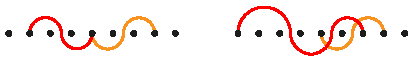
\includegraphics[scale=1.3]{incompatible}}
\caption{Some incompatible wiggly arcs: non pointed (left) and crossing (right).}
\label{fig:incompatible}
\end{figure}
\end{definition}

We consider sets of compatible wiggly arcs.
The following definitions are illustrated~in~\cref{fig:pseudodissections}.

\begin{definition}
A \defn{wiggly pseudodissection}~$D$ is a set of pairwise compatible wiggly arcs which contains the exterior wiggly arcs~$\alpha_\mathrm{top}$ and~$\alpha_\mathrm{bot}$. We denote by~$D^\circ \eqdef D \ssm \{\alpha_\mathrm{top}, \alpha_\mathrm{bot}\}$.
%
\begin{figure}[b]
\centerline{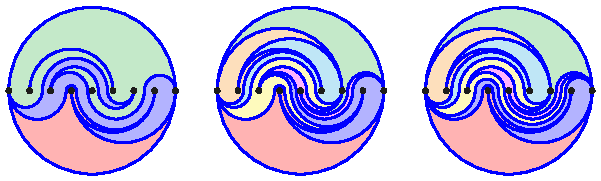
\includegraphics[scale=1.5]{pseudodissections}}
\caption{Three wiggly pseudodissections. The left one has three wiggly cells, of respective degrees $3$ (red), $8$ (green), and $4$ (blue). The other two have $7$ pseudotriangles, and are obtained from each other by flipping the wiggly arc separating their yellow and blue pseudotriangles.}
\label{fig:pseudodissections}
\end{figure}
\end{definition}

\begin{definition}
A wiggly pseudodissection~$D$ decomposes the digon bounded by~$\alpha_\mathrm{top}$ and~$\alpha_\mathrm{bot}$ into cells, that we call \defn{wiggly cells}.
The \defn{degree}~$\delta_c$ of a wiggly cell~$c$ is~$\delta_c \eqdef \beta_c/2+2\kappa_c-1$ where~$\beta_c$ is the number of arcs on the boundary of~$c$ (counted twice if they appear twice along the boundary of~$c$), and~$\kappa_c$ is the number of connected components of the boundary of~$c$.
A point~$p$ on the external boundary of~$c$ is a \defn{corner} (resp.~a \defn{hinge}) of~$c$ if~$c$ covers less (resp.~more) than half of any small disc centered at~$p$.
%The \defn{concave chains} of~$c$ are the maximal sequences of wiggly arcs on the external boundary of~$c$ connected by hinges of~$c$.
\end{definition}

\begin{remark}
\label{rem:degree}
Consider a wiggly cell~$c$ in a wiggly pseudodissection~$D$.
Note that~$\beta_c$ is always even as~$D$ is pointed, so that~$\beta_c/2$ is an integer.
Moreover, we have~$\beta_c \ge 2$ and~$\kappa_c \ge 1$, where at least one of the two inequalities is strict (as otherwise, the two wiggly arcs bounding~$c$ would coincide).
%We conclude that~$\delta_c = \beta_c/2+2\kappa_c-1 \ge 3$ with equality if and only if~$\beta_c = 4$ and~$\kappa_c = 1$.
We thus obtain on the one hand that~$\delta_c = \beta_c/2+2\kappa_c-1 \ge 3$ with equality if and only if~$\beta_c = 4$ and~$\kappa_c = 1$, and on the other hand that~$\beta_c/2+\kappa_c-1 \ge 2$.
\end{remark}

\begin{definition}
A \defn{wiggly pseudotriangle} (resp.~\defn{pseudoquadrangle}) is a wiggly cell of degree~$3$ (resp.~$4$).
\end{definition}

\begin{remark}
\label{rem:descriptionPseudotrianglesPseudoquadrangles}
As illustrated in \cref{fig:pseudotriangles}, a wiggly pseudotriangle~$t$ has no point in its interior and $4$ points on its boundary, $3$ corners and $1$ hinge.
%Hence, it has two corners oriented in the same direction, which we call the \defn{twin corners}.
As illustrated in \cref{fig:pseudoquadrangles}, a wiggly pseudoquadrangle~$q$ can have
\begin{enumerate}
\item either one point in its interior and~$2$ points on its boundary, both corners,
\item or no point in its interior and $6$ points on its boundary, $4$ corners and $2$ hinges. We then distinguish three situations, depending on the position of the two pairs~$p, p'$ of wiggly arcs incident to the two hinges of~$c$, as illustrated in \cref{fig:pseudoquadrangles} (where~$p$ and~$p'$ are colored in red and orange):
\begin{enumerate}[(a)]
\item those where $p$ and $p'$ are not consecutive along~$c$, and do not overlap vertically,
\item those where $p$ and $p'$ are not consecutive along~$c$, but overlap vertically.
\item those where~$p$ and~$p'$ are consecutive along~$c$,
\end{enumerate}
\end{enumerate}
%
\begin{figure}
\centerline{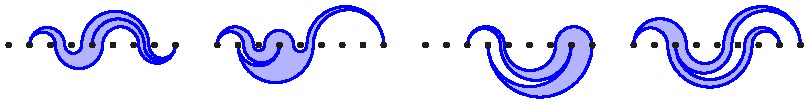
\includegraphics[scale=1.3]{pseudotriangles}}
\caption{Four wiggly pseudotriangles.}
\label{fig:pseudotriangles}
\end{figure}
%
\begin{figure}
\centerline{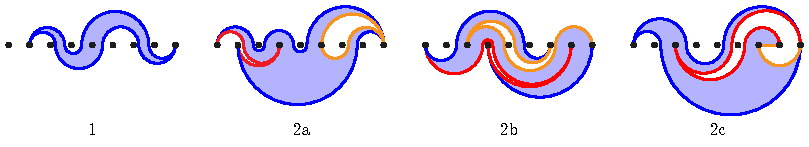
\includegraphics[scale=1.3]{pseudoquadrangles}}
\vspace{-.3cm}
\caption{Four types of wiggly pseudoquadrangles described in \cref{rem:descriptionPseudotrianglesPseudoquadrangles}.}
\label{fig:pseudoquadrangles}
\end{figure}
\end{remark}

\begin{proposition}
\label{prop:wigglyPseudotriangulations}
Any wiggly pseudodissection~$D$ contains at most~$2n-1$ internal wiggly arcs and at most~$n$ wiggly cells.
Moreover, the following are equivalent:
\begin{enumerate}[(i)]
\item all wiggly cells of~$D$ are wiggly pseudotriangles,
\item $D$ contains~$n$ wiggly cells and is connected,
\item $D$ contains $2n-1$ internal wiggly arcs,
\item $D$ is an inclusion maximal wiggly pseudodissection.
\end{enumerate}
We then say that~$D$ is a \defn{wiggly pseudotriangulation}.
\end{proposition}

\begin{proof}
Consider a wiggly pseudodissection~$D$ with~$\iota$ internal wiggly arcs, $\gamma$ wiggly cells, and~$\kappa$~connected components.
Euler's formula gives~$(n+2)-(\iota+2)+(\gamma+1)=(\kappa+1)$, hence~$\gamma=\iota+\kappa-n$.
Moreover, $\sum_{c \in D} \beta_c/2 = 1+\iota$ since each external (resp.~internal) wiggly arc bounds precisely one (resp.~two) wiggly cell of~$D$, and~${\sum_{c \in D} \big( \kappa_c-1 \big) = \kappa-1}$ since the boundary of each internal connected component of~$D$ is one of the internal connected components of the boundary of precisely one wiggly cell of~$D$.
As~$2 \le \beta_c/2+\kappa_c-1$ for any wiggly cell~$c$ by \cref{rem:degree}, we thus obtain that~$2\gamma \le \sum_{c \in D} (\beta_c/2+\kappa_c-1) = \iota+\kappa = \gamma+n$.
We conclude that~$\gamma \le n$ and~$\iota = \gamma-\kappa+n \le 2n-1$.

%Consider a wiggly pseudodissection~$D$ with~$\iota$ internal wiggly arcs, $\gamma$ wiggly cells, and~$\kappa$~connected components.
%Observe that~$\sum_{c \in D} \beta_c/2 = 1+\iota$ since each external (resp.~internal) wiggly arc bounds precisely one (resp.~two) wiggly cell of~$D$, and that~${\sum_{c \in D} \big( \kappa_c-1 \big) = \kappa-1}$ since the boundary of each internal connected component of~$D$ is one of the internal connected components of the boundary of precisely one wiggly cell of~$D$.
%As~$2 \le \beta_c/2+\kappa_c-1$ for any wiggly cell~$c$ by \cref{rem:degree}, we thus get~$2 \gamma \le \sum_{c \in D} (\beta_c/2+\kappa_c-1) = \iota+\kappa$.
%As~$D$ is a planar graph with~$v = n+2$ vertices, $e = \iota+2$ edges, $f = 1+\gamma$ faces, and $\kappa$ connected components, Euler's formula~$1+\kappa = v-e+f$ yields~$2(1+\kappa) = 2(n+2)-2(\iota+2)+2(1+\gamma) \le 2n-2\iota+2+\iota+\kappa$, so that~$\iota \le 2n-\kappa \le 2n-1$ and~$\gamma \le (\iota+\kappa)/2 \le n$.

To prove the second part of the statement, we show that~(i) $\Rightarrow$ (ii) $\Rightarrow$ (iii) $\Rightarrow$ (iv) $\Rightarrow$ (i).

\para{(i) $\Rightarrow$ (ii)}
For any wiggly cell~$c$, we have~$\delta_c = 3$, so that~$\beta_c = 4$ and~$\kappa_c = 1$ by \cref{rem:degree}, hence~$2 = \beta_c/2+\kappa_c-1$.
Therefore~$\kappa = 1$ ($D$ is connected) and~$2\gamma = \iota+1 = \gamma+n$, so that~$\gamma=n$.

\para{(ii) $\Rightarrow$ (iii)}
As $\gamma=n$ and~$\kappa=1$, we have~$\iota = \gamma+n-\kappa = 2n-1$.

%\para{(i) $\Rightarrow$ (ii)}
%We have~$\delta_c = 3$ for any wiggly cell~$c$.
%Hence~$\beta_c = 4$ and~$\kappa_c = 1$ by \cref{rem:degree}.
%Therefore~$2\gamma = \iota+1$ and~$\kappa = 1$ (so that~$D$ is connected).
%Applying Euler's formula as before, we get~$2 = (n+2)-(\iota+2)+(1+\gamma) = n-\gamma+2$, so that~$\gamma=n$.
%
%\para{(ii) $\Rightarrow$ (iii)}
%As $\gamma=n$ and~$\kappa=1$, we have~$2n = 2\gamma \le \iota+\kappa = \iota+1$, so that~$\iota = 2n-1$.

\para{(iii) $\Rightarrow$ (iv)}
If~$D$ already contains~$2n-1$ internal wiggly arcs, it has maximal cardinality among all wiggly pseudodissections, hence it is certainly inclusion maximal.

\para{(iv) $\Rightarrow$ (i)}
We now consider a wiggly pseudodissection~$D$ containing a wiggly cell~$c$ which is not a wiggly pseudotriangle, and we prove that~$D$ is not inclusion maximal.
%
Assume first that the external boundary of~$c$ is a digon bounded by the wiggly arcs~$\alpha \eqdef (i, j, A, B)$ and~$\alpha' \eqdef (i, j, A', B')$.
Denote by~$m$ the maximum of the points~$(A \symdif A') \cup (B \symdif B')$ located inside this digon (where~$\symdif$ denotes the symmetric difference).
Then the wiggly arc~$\beta \eqdef \big( i, m, {]i,m[} \cap (A \cup A'), {]i,m[} \cap (B \cap B') \big)$ is compatible with~$D$ (any wiggly arc incompatible with~$\beta$ crosses~$\alpha$ or~$\alpha'$) and is not in~$D$ (it connects the boundary of~$c$ with one of its internal connected components).
%Indeed, for any wiggly arc~$\gamma \eqdef (k, \ell, X, Y)$ inside~$c$, we have
%\begin{itemize}
%\item $i < k < \ell \le m$ so that~$\beta$ and~$\gamma$ are pointed,
%\item $Y \subseteq {]i,m[} \cap B \cap B'$ so that~$\beta$ and~$\gamma$ are non-crossing.
%\end{itemize}

Assume now that the external boundary of~$c$ is a not digon.
Consider a hinge~$j$ of~$c$.
Assume by symmetry that the boundary of~$c$ contains the two wiggly arcs~$\alpha \eqdef (i, j, A, B)$ and~$\alpha' \eqdef (i', j, A', B')$, such that~$\alpha$ is below~$\alpha'$. % (\ie $k \in A'$ or~$k' \in B$).
Let~$\gamma \eqdef (k, \ell, X, Y)$ denote the uppermost wiggly arc of the boundary of~$c$ such that~$j \in Y$ (it exists since~$j$ is a  hinge of~$c$), and let~$X' \eqdef {]j,\ell[} \cap X$ and~$Y' \eqdef {]j,\ell[} \cap Y$.
Then the two wiggly arcs~$\beta \eqdef \big( i, \ell, A \cup X', B \cup \{j\} \cup Y')$ and~$\beta' \eqdef \big( i', \ell, A'  \cup \{j\} \cup X', B \cup Y')$ are both compatible with~$D$ (any arc incompatible with~$\beta$ is incompatible with~$\alpha$ or~$\gamma$, and similarly for~$\beta'$) and cannot both belong to~$D$ (otherwise, $c$ would be a wiggly pseudotriangle bounded by~$\alpha, \alpha', \gamma', \gamma$).
\end{proof}

\begin{remark}
Note that in the proof of \cref{prop:wigglyPseudotriangulations}, we actually obtained that
\[
\sum_{c \in C} (\delta_c-3) = \sum_{c \in D} \beta_c/2 + 2 \sum_{c \in D} (\kappa_c-1) - 2\gamma = (1+\iota) + 2(\kappa-1) - 2(\iota+\kappa-n) = 2n-1-\iota.
\]
In other words, the number of wiggly arcs of~$D$ is $2n-1$ minus the number of wiggly cells of~$D$ which are not wiggly pseudotriangles.
\end{remark}

\begin{definition}
A \defn{wiggly diagonal} of a wiggly cell~$c$ is a wiggly arc inside~$c$ and compatible with~$c$.
\end{definition}

\begin{proposition}
\label{prop:diagonalsPseudoquadrangle}
Any wiggly pseudoquadrangle has exactly two wiggly diagonals.
Moreover, these two wiggly diagonals either cross precisely once, or are non pointed.
\end{proposition}

\begin{proof}
Depending on the four types of pseudoquadrangles described in \cref{rem:descriptionPseudotrianglesPseudoquadrangles}:
\begin{enumerate}
\item the two diagonals are the two wiggly arcs inside~$q$, incident to the point in the interior~of~$q$,
\item[(2a)] the two diagonals connect the two pairs of opposite corners of~$q$,
\item[(2b)] one of two diagonals connects two opposite corners of~$q$ while the other connects the two hinges~of~$q$,
\item[(2c)] one of the diagonals connects two opposite corners of~$q$ while the other connects an hinge of~$q$ to a corner of~$q$.
\end{enumerate}
See \cref{fig:diagonalsPseudoquadrangles} where the two diagonals appear in red and orange.
%
\begin{figure}[h]
\centerline{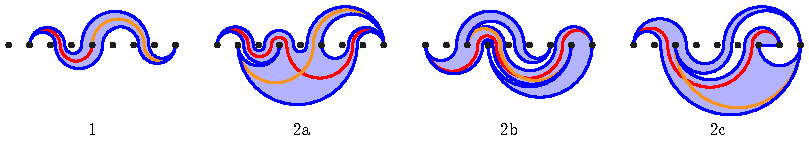
\includegraphics[scale=1.3]{diagonalsPseudoquadrangles}}
\caption{The two diagonals in each of the four types of wiggly pseudoquadrangles.} % described in \cref{rem:descriptionPseudotrianglesPseudoquadrangles}.}
\label{fig:diagonalsPseudoquadrangles}
\end{figure}
%Let~$q$ be a wiggly pseudoquadrangle.
%We distinguish two situations depending on~$\kappa(q)$:
%\begin{description}
%\item[$\kappa(q) = 1$] Then the boundary of~$c$ is a single wiggly hexagon, so that it has~$4$ concave points. We distinguish again two situations:
%	\begin{description}
%	\item 
%	\end{description}
%\item[$\kappa(q) = 2$] Then~$q$ is a digon bounded by two wiggly arcs~$(i, k, A, B \cup \{j\})$ and~$(i, k, A \cup \{j\}, B)$ for some~$1 < i < j < k \le n$ and~$A \sqcup B = {]i,j[} \cup{]j,k[}$. Hence, the only two wiggly arcs in the interior of~$q$ are~$(i, j, {]i,j[} \cap A, {]i,j[} \cap B)$ and~$(j, k, {]j,k[} \cap A, {]j,k[} \cap B)$, which are both compatible with~$q$ and are not pointed.
%\end{description}
\end{proof}

We are now ready to consider the wiggly flip graph and the wiggly complex.
The following definitions are illustrated in \cref{fig:wigglyComplex} when~$n = 2$.
%
\begin{figure}
\centerline{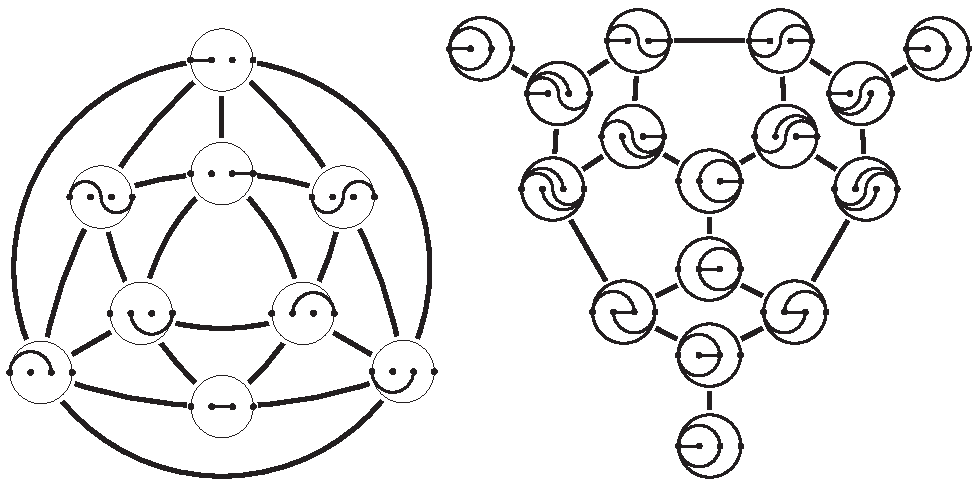
\includegraphics[scale=1.1]{wigglyComplex}}
\caption{The wiggly complex~$\wigglyComplex_2$ (left) and the wiggly flip graph~$\wigglyFlipGraph_2$ (right).}
\label{fig:wigglyComplex}
\end{figure}

\begin{definition}
The \defn{wiggly flip graph}~$\wigglyFlipGraph_n$ is the graph with a vertex for each wiggly pseudotriangulation, and with an edge between two wiggly pseudotriangulations~$T,T'$ if there are wiggly arcs~$\alpha \in T$ and~$\alpha' \in T'$ such that~$T \ssm \{\alpha\} = T' \ssm \{\alpha'\}$.
\end{definition}

\begin{proposition}
\label{prop:wigglyFlipGraph}
The wiggly flip graph~$\wigglyFlipGraph_n$ is regular of degree~$2n-1$.
\end{proposition}

\begin{proof}
Consider any internal wiggly arc~$\alpha$ of a wiggly pseudotriangulation~$T$.
Then~$Q \eqdef T \ssm \{\alpha\}$ contains~$n-2$ wiggly pseudotriangles and $1$ pseudoquadrangle~$q$.
By \cref{prop:diagonalsPseudoquadrangle}, $q$ admits precisely two wiggly diagonals, $\alpha$ and an other one~$\alpha'$.
As $\alpha'$ is inside~$q$ and compatible with~$c$, it is also compatible with~$Q$.
We obtain that~$T' \eqdef Q \cup \{\alpha'\}$ is the only wiggly pseudotriangulation other than~$T$ containing~$Q$.
\end{proof}

\begin{definition}
The \defn{wiggly complex}~$\wigglyComplex_n$ is the simplicial complex of pairwise pointed and non-crossing subsets of internal wiggly arcs.
In other words, it is the clique complex of the compatibility graph on internal wiggly arcs.
\end{definition}

\begin{proposition}
The wiggly complex~$\wigglyComplex_n$ is a flag pure $(2n-1)$-dimensional pseudomanifold without boundary.
\end{proposition}

\begin{proof}
It is a flag simplicial complex because it is a clique complex.
It is pure of dimension $2n-1$ by the implication (iv) $\Rightarrow$ (iii) of \cref{prop:wigglyPseudotriangulations}.
Finally, it is a pseudomanifold without boundary by \cref{prop:wigglyFlipGraph}.
\end{proof}

\begin{remark}
$\wigglyComplex_1$ contains two isolated points.
$\wigglyComplex_2$ is a simplicial $3$-dimensional associahedron (this coincidence fails for~$n > 2$).
Here are the first few $f$-vectors:
\begin{align*}
f(\wigglyComplex_1) & = (1, 2), \\
f(\wigglyComplex_2) & = (1, 9, 21, 14), \\
f(\wigglyComplex_3) & = (1, 24, 154, 396, 440, 176), \\
f(\wigglyComplex_4) & = (1, 55, 729, 4002, 10930, 15684, 11312, 3232), \\
f(\wigglyComplex_5) & = (1, 118, 2868, 28110, 140782, 400374, 673274, 662668, 352728, 78384),
\intertext{and the first few $h$-vectors:}
h(\wigglyComplex_1) & = (1, 1), \\
h(\wigglyComplex_2) & = (1, 6, 6, 1), \\
h(\wigglyComplex_3) & = (1, 19, 68, 68, 19, 1), \\
h(\wigglyComplex_4) & = (1, 48, 420, 1147, 1147, 420, 48, 1), \\
h(\wigglyComplex_5) & = (1, 109, 1960, 11254, 25868, 25868, 11254, 1960, 109, 1).
\end{align*}
\end{remark}

\begin{remark}
Note that the number of vertices of~$\wigglyComplex_n$ is the number~$\sum_{j = 0}^n 2^j (n+1-j)$ of wiggly arcs on~$n+2$ points.
The number of facets of~$\wigglyComplex_n$ is the number of wiggly pseudotriangulations of~$n+2$ points, which is a bit harder to compute.
For this, denote by $f_n(x)$ the polynomial where the coefficient of~$x^i$ is the number of wiggly pseudotriangulations of~$n+2$ points with~$i$ internal arcs ending at the last point~$n+1$.
For instance,
\begin{align*}
	f_0(x) & = 1 \\
	f_1(x) & = x + 1 \\
	f_2(x) & = 3 x^3 + 5 x^2 + 4 x + 2 \\
	f_3(x) & = 15 x^5 + 35 x^4 + 44 x^3 + 40 x^2 + 28 x + 14
\end{align*}
We use this additional variable~$x$ to obtain a recursive formula for~$f_n(x)$, discussing on the wiggly pseudotriangle~$t_n$ with a hinge at~$n$.
Namely, there are two types of wiggly pseudotriangulations of~$n+2$ points:
\begin{itemize}
\item those with the arc~$(n, n+1, \varnothing, \varnothing)$ are obtained from a wiggly pseudotriangulation of~$n+1$ points by choosing the position of the only corner of~$t_n$ which is not at~$n+1$,
\item those without the arc~$(n, n+1, \varnothing, \varnothing)$ are obtained from a wiggly pseudotriangulation of~$n+1$ points by choosing the positions of the two corners of~$t_n$ which are not at~$n+1$.
\end{itemize}
Hence we obtain for all~$n \ge 1$,
\[
f_{n}(x) = \frac{1}{(1 - x)^2} \big( f_{n-1}(1) + x^2 (2 x^2 - 2 x - 1) f_{n-1}(x) + x^4 (x - 1) f_{n-1}’(x) \big).
\]
This enables to quickly compute the generating series of the number of wiggly pseudotriangulations
\[
\sum_{n \ge 0} f(1) y^n = 1 + 2 y + 14 y^2 + 176 y^3 + 3232 y^4 + 78384 y^5 + 2366248 y^6 + 85534176 y^7 + 3602770400 y^8 + 
% 173300710720 y^9 + 9373542317760 y^10 + 563142033172480 y^11 + 37206559614499840 y^12 + 2681213937595142656 y^13 +
\dots
\]
\end{remark}

Finally, we will need the following observation, illustrated in \cref{fig:incompatible2}.

\begin{proposition}
\label{prop:uerp}
Let~$\alpha \eqdef (i, j, A, B)$ and~$\alpha' \eqdef (i', j', A', B')$ be two exchangeable wiggly arcs.
Then any wiggly arc compatible with both~$\alpha$ and~$\alpha'$ is also compatible with the wiggly~arcs:
\begin{itemize}
\item $\beta \eqdef (i, j', A \cup A', B \cup B' \cup \{j\})$ and~$\beta' \eqdef (i, j', A \cup A' \cup \{j\}, B \cup B')$ if~$\alpha$ and~$\alpha'$ are non pointed with~$j = i'$,
(In other words, ~$\beta$ and~$\beta'$ are the two wiggly arcs starting at~$\min(i,i')$ and ending at~$\max(j,j')$ which follow $\alpha$ on~$]i,j[$ and~$\alpha'$ on~$]i',j'[$.)
\item $\beta \eqdef \big( i, j', {]i,j'[} \ssm (B \cup B'), {]i,j'[} \cap (B \cup B') \big)$ and~$\beta' \eqdef \big( i', j, {]i',j[} \cap (A \cup A'), {]i',j[} \ssm (A \cup A') \big)$ if~$\alpha$ and~$\alpha'$ are crossing with~$i \in A'$ or~$i' \in B$.
(In other words, then~$\beta$ is the wiggly arc starting at~$i$ and ending at~$j'$ which follows the lower hull of~$\alpha$ and~$\alpha'$, and~$\beta'$ is the wiggly arc starting at~$i'$ and ending~at~$j$ which follows the upper hull of~$\alpha$ and~$\alpha'$.)
\end{itemize}
See \cref{fig:incompatible2} for illustrations.
%
\begin{figure}
\centering
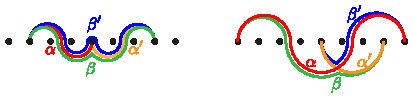
\includegraphics[scale=1.3]{incompatible2}
\caption{The arcs~$\beta$ and~$\beta'$ of \cref{prop:uerp}.}
\label{fig:incompatible2}
\end{figure}
%
(By exchanging~$\alpha$ and~$\alpha'$, similar statements hold if~$\alpha$ and~$\alpha'$ are non pointed with~$j = i'$, or if~$\alpha$ and~$\alpha'$ are crossing with~$i \in B'$ or~$i' \in A$.)
\end{proposition}

\begin{proof}
Any wiggly arc non pointed with~$\beta$ would be non pointed with~$\alpha$ or~$\alpha'$ (as the endpoints of~$\beta$ are endpoints of~$\alpha$ or~$\alpha'$).
Any wiggly arc crossing~$\beta$ would be either non pointed or crossing~$\alpha$ or~$\alpha'$ (as~$\beta$ follows~$\alpha$ or~$\alpha'$, except at the point~$j = i'$ in the first situation).
\end{proof}

%%%%%%%%%%%%

\subsection{Wiggly permutations and the wiggly lattice}
\label{subsec:wigglyPermutations}

We now consider wiggly permutations, defined as follows.

\begin{definition}
A \defn{wiggly permutation} is a permutation of~$[2n]$ which avoids the patterns:
\begin{itemize}
\item $(2j-1) \cdots i \cdots (2j)$ for~$j \in [n]$ and~$i < 2j-1$,
\item $(2j) \cdots k \cdots (2j-1)$ for~$j \in [n]$ and~$k > 2j$.
\end{itemize}
\end{definition}

\begin{example}
The wiggly permutations of~$[2]$ are~$12$ and~$21$.
The wiggly permutations of~$[4]$ are
\[
1234, 2134, 1342, 1243, 3421, 2143, 3412, 1432, 1423, 4321, 4213, 4312, 4132, 4123.
\]
%The wiggly permutations of~$[6]$ are
%\begin{gather*}
%123456, 213456, 134256, 124356, 123564, 123465, 342156, 214356, 213564, 213465, 341256, 143256, \\
%134562, 134265, 142356, 125643, 124365, 135642, 125634, 123654, 123645, 432156, 345621, 342165, \\
%421356, 215643, 214365, 356421, 215634, 213654, 213645, 431256, 341562, 341265, 413256, 143562, \\
%143265, 134652, 134625, 412356, 156423, 142365, 156243, 126543, 126435, 356412, 156342, 136542, \\
%156234, 126534, 126354, 136425, 126345, 435621, 432165, 346521, 346215, 564213, 421365, 562143, \\
%216543, 216435, 563421, 365421, 562134, 216534, 216354, 364215, 216345, 431562, 431265, 345612, \\
%341652, 341625, 413562, 413265, 156432, 143652, 143625, 136452, 564123, 412365, 561423, 165423, \\
%164235, 561243, 165243, 162543, 162435, 563412, 365412, 561342, 165342, 163542, 561234, 165234, \\
%162534, 162354, 364125, 163425, 162345, 564321, 436521, 436215, 364521, 654213, 642135, 652143, \\
%621543, 621435, 653421, 635421, 652134, 621534, 621354, 634215, 621345, 435612, 431652, 431625, \\
%346512, 346152, 346125, 564132, 413652, 413625, 561432, 165432, 164352, 164325, 364152, 163452, \\
%654123, 641235, 651423, 615423, 614235, 651243, 615243, 612543, 612435, 653412, 564312, 635412, \\
%651342, 615342, 613542, 651234, 615234, 612534, 612354, 634125, 613425, 612345, 654321, 643521, \\
%643215, 634521, 436512, 436152, 436125, 364512, 654132, 641352, 641325, 651432, 615432, 614352, \\
%614325, 634152, 613452, 654312, 643125, 643512, 643152, 634512.
%\end{gather*}
\end{example}

\begin{remark}
The numbers of wiggly permutations are given by
\[
\begin{array}{c|ccccccccc}
n & 1 & 2 & 3 & 4 & 5 & 6 & 7 & 8 & \dots \\
\hline
|\wigglyLattice_n| & 2 & 14 & 176 & 3232 & 78384 & 2366248 & 85534176 & 3602770400 & \dots
\end{array}
\]
\end{remark}

Recall that the \defn{inversion set} of a permutation~$\sigma$ of~$[2n]$ is the set
\[
\inv(\sigma) \eqdef \set{\big( \sigma(i), \sigma(j) \big)}{1 \le i < j \le 2n \text{ and } \sigma(i) > \sigma(j)}.
\]
We denote by~$\ninv(\sigma)$ the non-inversions of~$\sigma$, that is the complement of~$\inv(\sigma)$.
Note that~$\inv(\sigma)$ and~$\ninv(\sigma)$ are transitive: $\{(k,j), (j,i)\} \subseteq \inv(\sigma)$ implies~$(k,i) \in \inv(\sigma)$ for all~${1 \le i < j < k \le 2n}$, and similarly for~$\ninv$.
The inversion sets of wiggly permutations are characterized as follows.

\begin{lemma}
\label{lem:inversionSetsWigglyPermutations}
A permutation~$\sigma$ of~$[2n]$ is a wiggly permutation if and only if for all~$j \in [n]$,
\begin{itemize}
\item $(2j-1, i) \in \inv(\sigma)$ implies $(2j, i) \in \inv(\sigma)$ for all~$i < 2j-1$, and
\item $(k, 2j-1) \in \inv(\sigma)$ implies $(k, 2j) \in \inv(\sigma)$ for all~$k > 2j$.
\end{itemize}
A similar characterization holds for~$\ninv(\sigma)$ by exchanging~$2j-1$ and~$2j$.
\end{lemma}

\begin{proof}
Immediate as it precisely corresponds to the pattern avoidance description.
\end{proof}

The (left) \defn{weak order} on permutations of~$[2n]$ is defined as the inclusion order of their inversion sets.
Its cover relations are given by the exchanges of two entries at consecutive positions.
It is a (congruence uniform) lattice, and the join and meet satisfy
\[
\inv(\sigma \join \tau) = \big( \inv(\sigma) \cup \inv(\tau) \big)^\textrm{tc}
\qquad\text{and}\qquad
\ninv(\sigma \meet \tau) = \big( \ninv(\sigma) \cup \ninv(\tau) \big)^\textrm{tc}
\]
where~$X^\mathrm{tc}$ denotes the transitive closure of~$X$.

%The following statements are illustrated on \cref{fig:wigglyLattice}\,(right) when~${n = 2}$.
%
\begin{figure}
\centering
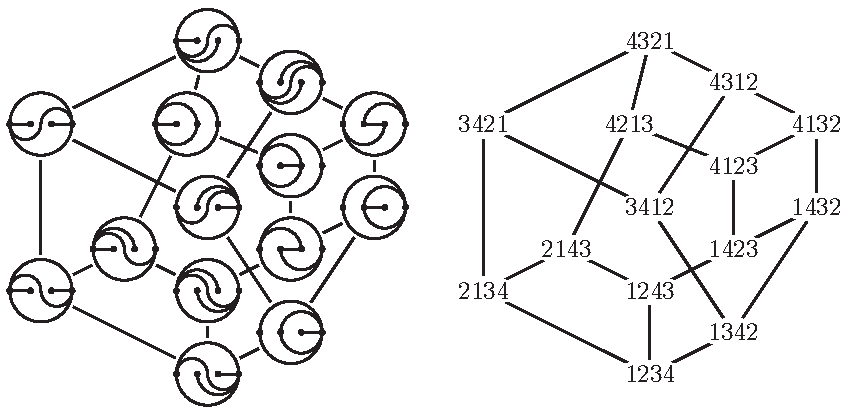
\includegraphics[scale=1.1]{wigglyFlipGraph}
\caption{The wiggly lattice~$\wigglyLattice_2$ on wiggly pseudotriangulations (left) and on wiggly permutations (right).}
\label{fig:wigglyLattice}
\end{figure}

\begin{proposition}
The wiggly permutations induce a sublattice of the weak order on permutations of~$[2n]$, that we call the \defn{wiggly lattice}~$\wigglyLattice_n$.
\end{proposition}

\begin{proof}
Consider two wiggly permutations~$\rho, \sigma$ of~$[2n]$, and let~$\tau = \rho \join \sigma$.
Assume that there is~$1 \le i < 2j-1 < 2n$ such that~$(2j-1, i) \in \inv(\tau)$.
As $\inv(\tau) = \big( \inv(\rho) \cup \inv(\sigma) \big)^\textrm{tc}$, there exist~$i \le i' < 2j-1$ such that~$(i', i) \in \inv(\tau)$ and~$(2j-1, i') \in \inv(\rho) \cup \inv(\sigma)$.
Since~$\rho$ and~$\sigma$ are wiggly permutations, we obtain by \cref{lem:inversionSetsWigglyPermutations} that~$(2j, i') \in \inv(\rho) \cup \inv(\sigma) \subseteq \inv(\tau)$.
As~$(i', i) \in \inv(\tau)$ and~$(2j, i') \in \inv(\tau)$ and~$\inv(\tau)$ is transitive, we conclude that~$(2j,i) \in \inv(\tau)$.
A similar argument shows that~$(k, 2j-1) \in \inv(\tau)$ implies~$(k, 2j) \in \inv(\tau)$ for all~$1 < 2j < k \le 2n$.
By \cref{lem:inversionSetsWigglyPermutations}, we conclude that~$\tau = \rho \join \sigma$ is a wiggly permutation.
The proof is similar for~$\rho \meet \sigma$, using $\ninv$ instead of~$\inv$.
\end{proof}

Recall that an \defn{ascent} (resp.~\defn{descent}) in a permutation~$\sigma$ is a position~$j$ such that~$\sigma(j) < \sigma(j+1)$ (resp.~$\sigma(j) > \sigma(j+1)$).

\begin{proposition}
Each wiggly permutation~$\sigma$ covers (resp.~is covered by) as many wiggly permutations as its number of descents (resp.~ascents), so that the cover graph of~$\wigglyLattice_n$ is regular of degree~$2n-1$.
\end{proposition}

\begin{proof}
Consider an ascent~$j$ of~$\sigma$.
Let~$i \eqdef \min \big( j, \sigma^{-1} \big( \sigma(j)+1 \big) \big)$ if~$\sigma(j)$ is odd, and $i \eqdef j$ otherwise.
Let~$k \eqdef \max \big( j+1, \sigma^{-1} \big( \sigma(j+1)+1 \big) \big)$ if~$\sigma(j+1)$ is odd, and $k \eqdef j+1$ otherwise.
Let~$\sigma^j \eqdef \sigma(1) \dots \sigma(i-1) \sigma(j+1) \dots \sigma(k) \sigma(i) \dots \sigma(j) \sigma(k+1) \dots \sigma(2n)$.
Then~$\sigma^j$ is the minimal wiggly permutation such that~$\inv(\sigma^j) \supseteq \inv(\sigma) \cup \big\{ \big( \sigma(j+1), \sigma(j) \big) \big\}$.
Moreover,~$\sigma^j \ne \sigma^{j'}$ for distinct ascents~$j \ne j'$.
As any permutation~$\sigma'$ larger than~$\sigma$ satisfies~${\inv(\sigma') \supseteq \inv(\sigma) \cup \{\sigma(j+1), \sigma(j)\}}$ for some ascent~$j$ of~$\sigma$, we thus obtain that~$j \to \sigma^j$ is a bijection from the ascents of~$\sigma$ to the wiggly permutations covering~$\sigma$.
The proof is symmetrical for the bijection from descents of~$\sigma$ to wiggly permutations covered by~$\sigma$.
\end{proof}

We close this section by the following conjecture (checked computationally up to~$n = 3$).

\begin{conjecture}
\label{conj:Hamiltonian}
The cover graph of the wiggly lattice~$\wigglyLattice_n$ is Hamiltonian.
\end{conjecture}

Note that unfortunately, wiggly permutations do not form a zigzag language in the sense of~\cite{HartungHoangMutzeWilliams} (which would have guarantied the existence of a Gray code).

%%%%%%%%%%%%

\subsection{Bijection}
\label{subsec:bijection}

We now prove that wiggly pseudotriangulations and wiggly permutations are in bijection, and that this bijection induces an isomorphism from the wiggly flip graph to the cover graph of the wiggly lattice.
The following two definitions are illustrated in \cref{fig:wigglyLattice,fig:bijection}.

\begin{figure}
\centerline{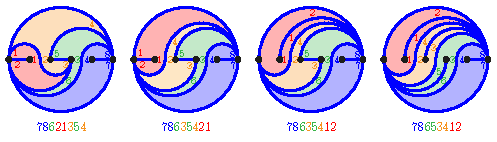
\includegraphics[scale=1.7]{bijection}}
\caption{The bijection between wiggly pseudotriangulations and wiggly permutations.}
\label{fig:bijection}
\end{figure}


\begin{definition}
\label{def:bijection1}
Consider a wiggly pseudotriangulation~$T$.
Rotating counterclockwise inside each wiggly pseudotriangle of~$T$, we label by~$2h-1$ (resp.~$2h+1$) the corner immediately preceding (resp.~following) the hinge~$h$ (the remaining corner remains unlabeled).
We define~$\Phi(T)$ as the permutation obtained by reading these labels from bottom to top, meaning that for each internal wiggly arc~$\alpha$ of~$T$, the label incident to~$\alpha$ and below~$\alpha$ appears just before the label incident to~$\alpha$ and above~$\alpha$.
\end{definition}

\begin{definition}
\label{def:bijection2}
For a wiggly permutation~$\sigma$ of~$[2n]$, we define~$\Psi(\sigma) \eqdef \set{\alpha(\sigma, k)}{k \in [2n-1]}$, where for~$k \in [2n-1]$, we have~$\alpha(\sigma, k) \eqdef \big( i, j, {]i,j[} \cap \sigma([k]), {]i,j[} \ssm \sigma([k]) \big)$ with
\[
i \eqdef \max \{0\} \cup \set{i \in [n]}{2i-1 \in \sigma([k]) \not\ni 2i} 
\;\text{and}\;
j \eqdef \min \{n+1\} \cup \set{j \in [n]}{2j \in \sigma([k]) \not\ni 2j-1} \!.
\]
\end{definition}

\begin{proposition}
The maps~$\Phi$ of \cref{def:bijection1} and $\Psi$ of \cref{def:bijection2} define inverse bijections between the wiggly pseudotriangulations and the wiggly permutations, which induce a graph isomorphism between the wiggly flip graph~$\wigglyFlipGraph_n$ and the cover graph of the wiggly lattice~$\wigglyLattice_n$.
\end{proposition}

\begin{proof}
%We first have to prove that~$\Phi$ and~$\Psi$ are well-defined.
\vincent{todo}
\end{proof}

%%%%%%%%%%%%%%%%%%%%%%%%%%%%%%%%%%%%%%

\section{Wiggly fan and wigglyhedron}
\label{sec:geometry}

%%%%%%%%%%%%

\subsection{Polyhedral geometry}
\label{subsec:polyhedralGeometry}

We refer to \cite{Ziegler-polytopes} for a reference on polyhedral geometry, and only remind the basic notions needed later in the paper.

A (polyhedral) \defn{cone} is the positive span~$\R_{\ge 0}\b{R}$ of a finite set~$\b{R}$ of vectors of~$\R^d$ or equivalently, the intersection of finitely many closed linear half-spaces of~$\R^d.$ 
The \defn{faces} of a cone are its intersections with its supporting hyperplanes. 
The \defn{rays} (resp.~\defn{facets}) are the faces of dimension~$1$ (resp.~ codimension~$1$).
A cone is \defn{simplicial} if its rays are linearly independent.
A (polyhedral) \defn{fan}~$\Fan$ is a set of cones such that any face of a cone of~$\Fan$ belongs to~$\Fan$, and any two cones of~$\Fan$ intersect along a face of both. 
A fan is \defn{essential} if the intersection of its cones is the origin, \defn{complete} if the union of its cones covers~$\R^d$, and \defn{simplicial} if all its cones are simplicial.

Note that a simplicial fan defines a simplicial complex on its rays (the simplices of the simplicial complex are the subsets of rays which span a cone of the fan).
Conversely, given a simplicial complex~$\Delta$ with ground set~$V$, one can try to realize it geometrically by associating a ray~$\b{r}_v$ of~$\R^d$ to each~$v \in V$, and the cone~$\R_{\ge 0}\b{R}_\triangle$ generated by the set~$\b{R}_\triangle \eqdef \set{\b{r}_v}{v \in \triangle}$ to each~$\triangle \in \Delta$.
To show that the resulting cones indeed form a fan, we will need the following statement, which can be seen as a reformulation of~\cite[Coro.~4.5.20]{DeLoeraRambauSantos}.

\begin{proposition}
\label{prop:characterizationFan}
Consider a closed simplicial $(d-1)$-dimensional pseudomanifold~$\Delta$ with ground set~$V$ and a set of vectors~$(\b{r}_v)_{v \in V}$ of~$\R^d$, and define~$\b{R}_\triangle \eqdef \set{\b{r}_v}{v \in \triangle}$ for any~$\triangle \in \Delta$.
Then the collection of cones~$\set{\R_{\ge 0}\b{R}_\triangle}{\triangle \in \Delta}$ forms a complete simplicial fan of~$\R^d$ if and~only~if
\begin{itemize}
\item there exists a vector~$\b{v}$ of~$\R^d$ contained in only one of the cones~$\R_{\ge 0}\b{R}_\triangle$ for~$\triangle \in \Delta$,
\item for any two adjacent facets~$\triangle, \triangle'$ of~$\Delta$ with~$\triangle \ssm \{v\} = \triangle' \ssm \{v'\}$, we have~$\lambda_v \lambda_{v'} > 0$~where
\[
\lambda_v \, \b{r}_v + \lambda_{v'} \, \b{r}_{v'} + \sum_{w \in \triangle \cap \triangle'} \lambda_w \, \b{r}_w = 0
\]
denotes the unique (up to rescaling) linear dependence on~$\b{R}_{\triangle \cup \triangle'}$.
\end{itemize}
\end{proposition}

A \defn{polytope} is the convex hull of finitely many points of~$\R^d$ or equivalently, a bounded intersection of finitely many closed affine half-spaces of~$\R^d$.
The \defn{faces} of a polytope are its intersections with its supporting hyperplanes.
The \defn{vertices} (resp.~\defn{edges}, resp.~\defn{facets}) are the faces of dimension~$0$ (resp.~dimension~$1$, resp.~codimension~$1$).

The \defn{normal cone} of a face~$\polytope{F}$ of a polytope~$\polytope{P}$ is the cone generated by the normal vectors to the supporting hyperplanes of~$\polytope{P}$ containing~$\polytope{F}$.
Said differently, it is the cone of vectors~$\b{c}$ of~$\R^d$ such that the linear form~$\b{x} \mapsto \dotprod{\b{c}}{\b{x}}$ on~$\polytope{P}$ is maximized by all points of the face~$\polytope{F}$.
The \defn{normal fan} of~$\polytope{P}$ is the set of normal cones of all its faces.

Consider now a complete simplicial fan~$\Fan$ of~$\R^d$ with rays~$(\b{r}_v)_{v \in V}$ and cones~$\R_{\ge 0} \b{R}_\triangle$ for~${\triangle \in \Delta}$, where~$\b{R}_\triangle \eqdef \set{\b{r}_v}{v \in \triangle}$ as in \cref{prop:characterizationFan}.
To realize the fan~$\Fan$, one can try to pick a height vector~$\b{h} \eqdef (h_v)_{v \in V} \in \R^V$ and consider the polytope
\(
\polytope{P}_{\b{h}} \eqdef \set{\b{x} \in \R^d}{\dotprod{\b{r}_v}{\b{x}} \le h_v \text{ for all } v \in V}.
\)
The following classical statement characterizes the height vectors~$\b{h}$ for which the fan~$\Fan$ is the normal fan of this polytope~$\polytope{P}_{\b{h}}$.
We borrow the formulation from~\cite[Lem.~2.1]{ChapotonFominZelevinsky}.

\begin{proposition}
\label{prop:characterizationPolytopalFan}
Let~$\Fan$ be an essential complete simplicial fan in~$\R^n$ with rays~$(\b{r}_v)_{v \in V}$ and cones~$\R_{\ge 0} \b{R}_\triangle$ for~$\triangle \in \Delta$.
Then the following are equivalent for any height vector~$\b{h} \in \R^V$:
\begin{itemize}
\item The fan~$\Fan$ is the normal fan of the polytope~$\polytope{P}_{\b{h}} \eqdef \set{\b{x} \in \R^d}{\dotprod{\b{r}_v}{\b{x}} \le h_v \text{ for all } v \in V}$.
\item For two adjacent facets~$\triangle, \triangle'$ of~$\Delta$ with~$\triangle \ssm \{v\} = \triangle' \ssm \{v'\}$, the height vector~$\b{h}$ satisfies the \defn{wall crossing inequality}
\[
\lambda_v \, h_v + \lambda_{v'} \, h_{v'} + \sum_{w \in \triangle \cap \triangle'} \lambda_w \, h_w > 0
\]
where
\[
\lambda_v \, \b{r}_v + \lambda_{v'} \, \b{r}_{v'} + \sum_{w \in \triangle \cap \triangle'} \lambda_w \, \b{r}_w = 0
\]
denotes the unique linear dependence on~$\b{R}_{\triangle \cup \triangle'}$ such that~$\lambda_v + \lambda_{v'} = 2$.
\end{itemize}
\end{proposition}

We denote by~$(\b{e}_i)_{i \in [d]}$ the standard basis of~$\R^d$.
For~$I \subseteq [d]$, we define~$\one_I \eqdef \sum_{i \in I} \b{e}_i$, and we often shorten~$\one_{[d]}$ by~$\one_d$.
We denote by~$\HH_d$ the hyperplane of~$\R^d$ defined by the equation~$\dotprod{\b{x}}{\one_d} = 0$, and we denote by~$\pi : \R^d \to \HH$ the orthogonal projection on~$\HH_d$, that is~$\pi(\b{x}) \eqdef \b{x} - (\dotprod{\b{x}}{\one_d} / d) \one_d$.

%%%%%%%%%%%%

\subsection{$\b{g}$-vectors and $\b{c}$-vectors}
\label{subsec:gcvectors}

We now define two families of vectors, illustrated in \cref{fig:pseudotriangulationMatrices}.
%
\begin{figure}
\centerline{\raisebox{-1.8cm}{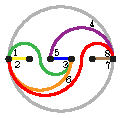
\includegraphics[scale=2]{pseudotriangulationMatrices}} \quad \scalebox{.9}{
\(
\begin{blockarray}{ccccccccc}
	& & {\color{brown} \bullet} & {\color{red} \bullet} & {\color{orange} \bullet} & {\color{yellow} \bullet} & {\color{green} \bullet} & {\color{blue} \bullet} & {\color{violet} \bullet} \\
	\begin{block}{c@{\hspace*{-.1cm}}c(ccccccc)}
	1 & & 0 & \!\! -1 \!\! & \!\! -1 \!\! & \!\! -1 \!\! & 1 & 0 & 0 \\
	2 & & 0 & \!\! -1 \!\! & \!\! -1 \!\! & 1 & 1 & 0 & 0 \\
	3 & & 0 & \!\! -1 \!\! & \!\! -1 \!\! & 0 & \!\! -1 \!\! & 1 & 1 \\
	4 & & 0 & \!\! -1 \!\! & \!\! -1 \!\! & 0 & \!\! -1 \!\! & \!\! -1 \!\! & \!\!\! -1 \! \\
	5 & & 0 & \!\! -1 \!\! & \!\! -1 \!\! & 0 & \!\! -1 \!\! & \!\! -1 \!\! & 1 \\
	6 & & 0 & \!\! -1 \!\! & 1 & 0 & 1 & 1 & 1 \\
	7 & & 1 & 1 & 0 & 0 & 0 & 0 & 1 \\
	8 & & \! -1 \!\!\! & 1 & 0 & 0 & 0 & 0 & 1 \\
	\end{block}
	& & & & \multicolumn{2}{c}{$\hat{\b{g}}(T)$} & &
\end{blockarray}
%
\qquad
%
\begin{blockarray}{ccccccccc}
	& & {\color{brown} \bullet} & {\color{red} \bullet} & {\color{orange} \bullet} & {\color{yellow} \bullet} & {\color{green} \bullet} & {\color{blue} \bullet} & {\color{violet} \bullet} \\
	\begin{block}{c@{\hspace*{-.1cm}}c(ccccccc)}
	1 & & 0 & 0 & \!\! -1 \!\! & 2 & 1 & 0 & 0 \\
	2 & & 0 & 0 & \!\! -1 \!\! & \!\! -2 \!\! & 1 & 0 & 0 \\
	3 & & 0 & 0 & \!\! -1 \!\! & 0 & \!\! -1 \!\! & 2 & 0 \\
	4 & & 0 & 0 & 1 & 0 & \!\! -1 \!\! & 0 & \!\! -2 \!\! \\
	5 & & 0 & \!\! -1 \!\! & 0 & 0 & 0 & \!\! -2 \!\! & 2 \\
	6 & & 0 & \!\! -1 \!\! & 2 & 0 & 0 & 0 & 0 \\
	7 & & 2 & 1 & 0 & 0 & 0 & 0 & 0 \\
	8 & & \! -2 \!\!\! & 1 & 0 & 0 & 0 & 0 & 0 \\
	\end{block}
	& & & & \multicolumn{2}{c}{$4\b{c}(T)$} & &
\end{blockarray}
\)
}}
\caption{The $\b{g}$-matrix and $\b{c}$-matrix of a wiggly pseudotriangulation~$T$. The $i$th column of these matrices are the $\b{g}$-vector~$\b{g}(\alpha)$ and $\b{c}$-vector~$\b{c}(\alpha, T)$ of the $i$th wiggly arc~$\alpha$ of~$T$ (ordered from bottom to top). The colors of the columns match the colors of the wiggly arcs.}
\label{fig:pseudotriangulationMatrices}
\end{figure}

\begin{definition}
\label{def:gvectors}
The \defn{$\b{g}$-vector}~$\b{g}(\alpha)$ of a wiggly arc~$\alpha \eqdef (i, j, A, B)$ is defined as the projection~$\pi \big( \hat{\b{g}}(\alpha) \big)$ of the vector~$\hat{\b{g}}(\alpha) \eqdef \one_{\alpha^+} - \one_{\alpha^-}$ where
\begin{align*}
\alpha^+ & \eqdef \big(\{2i-1, 2j\} \ssm \{-1, 2n+2\} \big) \cup \set{2a-1}{a \in A} \cup \set{2a}{a \in A},
\\
\alpha^- & \eqdef \big(\{2i, 2j-1\} \ssm \{0, 2n+1\} \big) \cup \set{2b-1}{b \in B} \cup \set{2b}{b \in B}.
\end{align*}
If we place the coordinate~$2p-1$ on the left and the coordinate~$2p$ on the right of point~$p$, then~$\b{g}(\alpha)$ has a $1$ outside its two endpoints and on both sides of points in~$A$, and a~$-1$ inside its two endpoints and on both sides of points in~$B$.
Note that ${\hat{\b{g}} \big( (0, n+1, [n], \varnothing) \big) = \one_{2n} = - \hat{\b{g}} \big( (0, n+1, \varnothing, [n]) \big)}$, so that~${\b{g} \big( (0, n+1, [n], \varnothing) \big) = \b{0} = \b{g} \big( (0, n+1, \varnothing, [n]) \big)}$.
We define~$\b{g}(D) \eqdef \set{\b{g}(\alpha)}{\alpha \in D^\circ}$ for a set~$D$ of wiggly arcs.
\end{definition}

\begin{definition}
\label{def:cvectors}
Consider a wiggly pseudotriangulation~$T$, and label the corners as in \cref{def:bijection1}.
Consider an interior wiggly arc~$\alpha$ in a wiggly pseudotriangulation~$T$, denote by~$u$ and~$v$ the labels incident to~$\alpha$ and respectively below and above~$\alpha$, and let~$\bar u \eqdef \lceil u/2 \rceil$ and~$\bar v \eqdef \lceil v/2 \rceil$.
The \defn{$\b{c}$-vector} of~$\alpha$ in~$T$ is the vector~$\b{c}(\alpha, T)$ with coordinates
\begin{itemize}
\item $\b{c}(\alpha, T)_{2w-1} = - \b{c}(\alpha, T)_{2w} = (-1)^{w \in A} (-1)^{u>v}/4$ for all~$w$ strictly between~$\bar u$ and~$\bar v$,
\item $\b{c}(\alpha, T)_u = 1/2$ if~$\bar v$ and the wiggly arcs incident to~$\bar u$ are on the same side of~$\bar u$, and $\b{c}(\alpha, T)_{2\bar u-1} = \b{c}(\alpha, T)_{2\bar u} = 1/4$ otherwise,
\item $\b{c}(\alpha, T)_v = -1/2$ if~$\bar u$ and the wiggly arcs incident to~$\bar v$ are on the same side of~$\bar v$, and $\b{c}(\alpha, T)_{2\bar v-1} = \b{c}(\alpha, T)_{2\bar v} = -1/4$ otherwise,
\item $\b{c}(\alpha, T)_w = 0$ for all other coordinates.
\end{itemize}
Set~$\b{c}(T) \eqdef \set{\b{c}(\alpha, T)}{\alpha \in T^\circ}$
\end{definition}

\begin{proposition}
\label{prop:dualBases}
For any wiggly pseudotriangulation~$T$, the sets~$\b{g}(T)$ and~$\b{c}(T)$ are dual bases~of~$\HH_{2n}$.
\end{proposition}

\begin{proof}
We first prove that~$\dotprod{\hat{\b{g}}(\alpha)}{\b{c}(\alpha', T)} = \delta_{\alpha, \alpha'}$ for any~$\alpha, \alpha' \in T$, where~$\delta$ is the Kronecker~$\delta$.
\vincent{todo}

Note that, with~$\alpha = (0, n+1, [n], \varnothing)$, it implies that~$\dotprod{\one_{2n}}{\b{c}(\alpha', T)} = 0$ for any~${\alpha' \in T}$.
Hence, we obtain that~$\dotprod{\b{g}(\alpha)}{\b{c}(\alpha', T)} = \dotprod{\pi(\hat{\b{g}}(\alpha))}{\b{c}(\alpha', T)} = \dotprod{\hat{\b{g}}(\alpha)}{\b{c}(\alpha', T)} = \delta_{\alpha, \alpha'}$ for any~$\alpha, \alpha' \in T$.
We conclude that~$\b{g}(T) \eqdef \set{\b{g}(\alpha)}{\alpha \in T^\circ}$ and~$\b{c}(T) \eqdef \set{\b{c}(\alpha, T)}{\alpha \in T^\circ}$ form dual bases of~$\HH_{2n}$.
\end{proof}

%%%%%%%%%%%%

\subsection{Wiggly fan}
\label{subsec:wigglyFan}

We now show that the $\b{g}$-vectors of \cref{def:gvectors} support a polyhedral fan realization of the wiggly complex~$\wigglyComplex_n$.

\begin{theorem}
\label{thm:wigglyFan}
The collection of cones~$\R_{\ge 0} \langle \b{g}(A) \rangle$ for all~$A$ in the wiggly complex~$\wigglyComplex_n$ forms a complete simplicial fan of~$\HH_{2n}$, called \defn{wiggly fan}~$\wigglyFan_n$.
\end{theorem}

To prove \cref{thm:wigglyFan}, we just need to check the conditions of \cref{prop:characterizationFan}.
We first find a vector contained in the cone~$\R_{\ge 0} \langle \b{g}(T) \rangle$ for a single wiggly pseudotriangulation~$T$.

\begin{lemma}
\label{lem:-+...-+}
Let~$\b{v} \eqdef \sum_{k \in [n]} (\b{e}_{2k} - \b{e}_{2k-1}) = (-1, 1, \dots, -1, 1)$, let~$\alpha_0 \eqdef (0, 1, \varnothing, \varnothing)$, and let~$\underline{\alpha}_i \eqdef (0, i+1, [i], \varnothing)$ and~$\overline{\alpha}_i \eqdef (0, i+1, \varnothing, [i])$ for all~${i \in [n]}$.
Then~$\{\alpha_0\} \cup \bigcup_{i \in [n]} \{\underline{\alpha}_i, \overline{\alpha}_i\}$ is the only wiggly pseudotriangulation~$T$ such that~$\b{v} \in \R_{\ge 0} \langle \b{g}(T) \rangle$.
\end{lemma}

\begin{proof}
Observe first that, for any wiggly arc~$\alpha \eqdef (i, j, A, B)$ and any~$k \in [n]$, we have
%\begin{itemize}
%\item $\hat{\b{g}}(\alpha)_{2k-1} - \hat{\b{g}}(\alpha)_{2k} = 1$ if~$k = i$, $-1$ if~$k = j$, and~$0$ otherwise,
%\item $\hat{\b{g}}(\alpha)_{2k-1} + \hat{\b{g}}(\alpha)_{2k} = 2$ if~$k \in A$, $-2$ if~$k \in B$, and~$0$ otherwise.
%\end{itemize}
\[
\hat{\b{g}}(\alpha)_{2k-1} - \hat{\b{g}}(\alpha)_{2k} = \begin{cases} 1 & \text{if~$k = i$,} \\ -1 & \text{if~$k = j$,} \\ 0 & \text{otherwise}, \end{cases}
\qquad\text{and}\qquad
\hat{\b{g}}(\alpha)_{2k-1} + \hat{\b{g}}(\alpha)_{2k} = \begin{cases} 2 & \text{if~$k \in A$,} \\ -2 & \text{if~$k \in B$,} \\ 0 & \text{otherwise}. \end{cases}
\]

Assume now that~$\b{v} = \sum_\alpha \lambda_\alpha \, \hat{\b{g}}(\alpha)$ where the sum ranges over all wiggly arcs~$\alpha$ for some positive scalars~$\lambda_\alpha \ge 0$ such that~$\lambda_\alpha \cdot \lambda_{\alpha'} = 0$ for all incompatible wiggly arcs~$\alpha$ and~$\alpha'$.
For~$k \in [n]$, let~$\underline{\Lambda}_k$ (resp.~$\overline{\Lambda}_k$) denote the sum of~$\lambda_\alpha$ over the wiggly arcs~$\alpha \eqdef (i, j, A, B)$ with~$k \in A$ (resp.~$k \in B$).
Note that~$\underline{\Lambda}_k = \overline{\Lambda}_k$ since~$0 = \b{v}_{2k-1} + \b{v}_{2k} = \sum_\alpha \lambda_\alpha \big( \hat{\b{g}}(\alpha)_{2k-1} + \hat{\b{g}}(\alpha)_{2k} \big) = 2\underline{\Lambda}_k - 2\overline{\Lambda}_k$.

As~$\b{v}_1 - \b{v}_2 = -2$ and~$\hat{\b{g}}(\alpha)_1 - \hat{\b{g}}(\alpha)_2 \ge 0$ except if~$\alpha = \alpha_0$, we have~$\lambda_{\alpha_0} > 0$, and thus~$\lambda_{\alpha} = 0$ for all wiggly arcs~$\alpha$ starting at~$1$.
%As~$\b{g}(\alpha)_1 - \b{g}(\alpha)_2 = 0$ for all wiggly arcs~$\alpha$ with no endpoint at~$1$, we thus obtain that~$\lambda_{\alpha_0} = 1$.
We then prove by induction on~$i \in [n-1]$ that~$\lambda_{\underline{\alpha}_i} \cdot \lambda_{\overline{\alpha}_i} > 0$ and that~$\lambda_\alpha = 0$ for all wiggly arcs starting at~$i+1$.
Consider~$i \in [n-1]$ and assume that we proved it for~$i-1$.
As~$\smash{\lambda_{\underline{\alpha}_{i-1}} \cdot \lambda_{\overline{\alpha}_{i-1}} > 0}$, we already have~$\lambda_\alpha = 0$ for all wiggly arcs~$\alpha$ ending at~$i+1$, except if~$\alpha \in \{\underline{\alpha}_i, \overline{\alpha}_i\}$.
As~$\b{v}_{2i+1} - \b{v}_{2i+2} = -2$, this implies that~$\smash{\lambda_{\underline{\alpha}_i} + \lambda_{\overline{\alpha}_i} = 1}$.
This already implies that~$\lambda_{\alpha} = 0$ for all wiggly arcs~$\alpha$ starting at~$i+1$.
Moreover, assume for instance that~$\lambda_{\overline{\alpha}_i} > 0$.
Hence, $\lambda_\alpha = 0$ for all wiggly arcs~$\alpha \eqdef (i, j, A, B)$ with~$i \in A$ and~$i+1 \in B$.
We thus obtain that~$\underline{\Lambda}_i - \lambda_{\underline{\alpha}_i} \le \underline{\Lambda}_{i+1}$ and~$\overline{\Lambda}_i - \lambda_{\overline{\alpha}_i} \ge \overline{\Lambda}_{i+1}$.
As~$\underline{\Lambda}_i = \overline{\Lambda}_i$ and~$\underline{\Lambda}_{i+1} = \overline{\Lambda}_{i+1}$, we thus obtain that~$\lambda_{\underline{\alpha}_i} \ge \lambda_{\overline{\alpha}_i} > 0$, hence that~$\lambda_{\underline{\alpha}_i} \cdot \lambda_{\overline{\alpha}_i} > 0$.
We conclude that~$\lambda_\alpha = 0$ for all wiggly arcs~$\alpha$ except if~$\alpha = \alpha_0$ or~$\alpha \in \{\underline{\alpha}_i, \overline{\alpha}_i\}$ for some~$i \in [n]$.

Consider now a wiggly pseudotriangulation~$T$ such that~$\b{v} \in \R_{\ge 0} \langle \b{g}(T) \rangle$.
Write~$\b{v} = \sum_{\alpha \in T^\circ} \lambda_\alpha \, \b{g}(\alpha)$ with~$\lambda_\alpha \ge 0$ for all~$\alpha \in T^\circ$.
Let~$\mu \eqdef \sum_{\alpha \in T^\circ} \lambda_\alpha \dotprod{\hat{\b{g}}(\alpha)}{\one_{2n}}$.
As~$\b{v} = \sum_{\alpha \in T^\circ} \lambda_\alpha \, \hat{\b{g}}(\alpha) - \mu \, \one_{2n}$ and~$\one_{2n} = \hat{\b{g}} \big( (0, n+1, [n], \varnothing) \big) = - \hat{\b{g}} \big( (0, n+1, \varnothing, [n]) \big)$, we thus conclude from the previous paragraph that~$T = \{\alpha_0\} \cup \bigcup_{i \in [n]} \{\underline{\alpha}_i, \overline{\alpha}_i\}$.
\end{proof}

We now describe the unique linear dependence between the $\b{g}$-vectors of two adjacent facets of the wiggly complex~$\wigglyComplex_n$.
The following statement is illustrated in \cref{fig:linearDependences}.

\begin{lemma}
\label{lem:linearDependences}
Let~$T$ and~$T'$ be two adjacent wiggly pseudotriangulations with~$T \ssm \{\alpha\} = T' \ssm \{\alpha'\}$, and let~$\beta$ and~$\beta'$ be the wiggly arcs defined in \cref{prop:uerp}.
Then~$\{\beta, \beta'\} \in T \cap T'$ and
\begin{itemize}
\item if $\alpha$ and~$\alpha'$ are not pointed, then~$\b{g}(\alpha) + \b{g}(\alpha') = \big( \b{g}(\beta) + \b{g}(\beta') \big) / 2$,
\item if~$\alpha$ and~$\alpha'$ are crossing, then~${\b{g}(\alpha) + \b{g}(\alpha') = \b{g}(\beta) + \b{g}(\beta')}$.
\end{itemize}
%Let~$\alpha \eqdef (i, j, A, B)$ and~$\alpha' \eqdef (i', j', A', B')$ be two exchangeable wiggly arcs, and let~$T$ and~$T'$ be two adjacent wiggly pseudotriangulations such that~$T \ssm \{\alpha\} = T' \ssm \{\alpha'\}$.
%Then
%\begin{description}
%\item[if $\alpha$ and~$\alpha'$ are not pointed] Assume without loss of generality that~$i' = j$, and consider %the wiggly arcs~
%$\beta \eqdef (i, j', A \cup A', B \cup B' \cup \{j\})$ and~$\beta' \eqdef (i, j', A \cup A' \cup \{j\}, B \cup B')$.
%(In other words, ~$\beta$ and~$\beta'$ are the two wiggly arcs starting at~$\min(i,i')$ and ending at~$\max(j,j')$ which follow $\alpha$ on~$]i,j[$ and~$\alpha'$ on~$]i',j'[$.)
%Then~$\{\beta, \beta'\} \in T \cap T'$ and~$\b{g}(\alpha) + \b{g}(\alpha') = \big( \b{g}(\beta) + \b{g}(\beta') \big) / 2$.
%\item[if~$\alpha$ and~$\alpha'$ are crossing] Assume without loss of generality that~$i \in A'$ or~$i' \in B$, and consider %the wiggly arcs~
%$\beta \eqdef \big( i, j', {]i,j'[} \ssm (B \cup B'), {]i,j'[} \cap (B \cup B') \big)$ and~$\beta' \eqdef \big( i', j, {]i',j[} \cap (A \cup A'), {]i',j[} \ssm (A \cup A') \big)$. \linebreak
%(In other words, if~$p$ denotes the crossing point of~$\alpha$ and~$\alpha'$, then~$\beta$ is the wiggly arc starting at~$i$ and ending at~$j'$ which follows~$\alpha$ on~$]i,p[$ and~$\alpha'$ on~$]p,j'[$, and~$\beta'$ is the wiggly arc starting at~$i'$ and ending~at~$j$ which follows~$\alpha$ on~$]i',p[$ and~$\alpha$ on~$]p,j[$.)
%Then~${\{\beta, \beta'\} \in T \cap T'}$ and~${\b{g}(\alpha) + \b{g}(\alpha') = \b{g}(\beta) + \b{g}(\beta')}$.
%\end{description}
\end{lemma}

\begin{proof}
In both situations, we will just prove that the same linear dependence holds on the vectors~$\hat{\b{g}}(\alpha), \hat{\b{g}}(\alpha'), \hat{\b{g}}(\beta), \hat{\b{g}}(\beta')$, which will imply the statement as~$\pi$ is a linear map.

If~$\alpha$ and~$\alpha'$ are non pointed with~$i' = j$, then we have
\[
\alpha^+ \sqcup \alpha'^+ = \beta^+ \sqcup \{2j-1, 2j\} = \beta'^+
\qquad\text{and}\qquad 
\alpha^- \sqcup \alpha'^- = \beta^- = \beta'^- \sqcup \{2j-1, 2j\}.
\]
We thus obtain that
\[
\one_{\alpha^+} + \one_{\alpha'^+} = \one_{\beta^+} + \b{e}_{2j-1} + \b{e}_{2j} = \one_{\beta'^+}
\qquad\text{and}\qquad 
\one_{\alpha^-} + \one_{\alpha'^-} = \one_{\beta^-} = \one_{\beta'^-} + \b{e}_{2j-1} + \b{e}_{2j}.
\]
hence
\begin{align*}
2 \big( \hat{\b{g}}(\alpha) + \hat{\b{g}}(\alpha') \big)
& = 2(\one_{\alpha^+} - \one_{\alpha^-}) + 2(\one_{\alpha'^+} - \one_{\alpha'^-})
= 2(\one_{\alpha^+} + \one_{\alpha'^+}) - 2(\one_{\alpha^-} + \one_{\alpha'^-}) \\
& = (\one_{\beta^+} + \one_{\beta'^+} + \b{e}_{2j-1} + \b{e}_{2j}) - (\one_{\beta^-} + \one_{\beta'^-} + \b{e}_{2j-1} + \b{e}_{2j}) \\
& = (\one_{\beta^+} + \one_{\beta'^+}) - (\one_{\beta^-} + \one_{\beta'^-})
= (\one_{\beta^+} - \one_{\beta^-}) + (\one_{\beta^-} + \one_{\beta'^-})
= \hat{\b{g}}(\beta) + \hat{\b{g}}(\beta').
\end{align*}

If~$\alpha$ and~$\alpha'$ are crossing with~$i \in A'$ or~$i' \in B$, then we have
\begin{gather*}
\alpha^+ \cup \alpha'^+ = \beta^+ \cup \beta'^+ \qquad\text{and}\qquad \alpha^+ \cap \alpha'^+ = \beta^+ \cap \beta'^+, \\
\alpha^- \cup \alpha'^- = \beta^- \cup \beta'^- \qquad\text{and}\qquad \alpha^- \cap \alpha'^- = \beta^- \cap \beta'^-.
\end{gather*}
We thus obtain that
\[
\one_{\alpha^+} + \one_{\alpha'^+} = \one_{\alpha^+ \cup \alpha'^+} + \one_{\alpha^+ \cap \alpha'^+} = \one_{\beta^+ \cup \beta'^+} + \one_{\beta^+ \cap \beta'^+} = \one_{\beta^+} + \one_{\beta'^+}
\]
and similarly~$\one_{\alpha^-} + \one_{\alpha'^-} = \one_{\beta^-} + \one_{\beta'^-}$, so that~$\hat{\b{g}}(\alpha) + \hat{\b{g}}(\alpha') =\hat{\b{g}}(\beta) + \hat{\b{g}}(\beta')$.
\end{proof}

\begin{proof}[Proof of \cref{thm:wigglyFan}]
Directly follows from \cref{prop:characterizationFan,lem:-+...-+,lem:linearDependences}.
\end{proof}

\begin{remark}
The wiggly fan coarsens the $\b{c}$-vector fan.
\vincent{todo}
\end{remark}

%%%%%%%%%%%%

\subsection{Wigglyhedron}
\label{subsec:wigglyhedron}

We now construct the wigglyhedron illustrated in \cref{fig:wigglyhedron} when~${n = 2}$.
%
\begin{figure}[t]
\centering
\begin{tikzpicture}%
	[x={(0.681462cm, -0.327528cm)},
	y={(0.731633cm, 0.326817cm)},
	z={(-0.017949cm, 0.886519cm)},
	scale=.500000,
	back/.style={color=blue, thin},
	edge/.style={color=blue, very thick, },
	facet/.style={fill=blue,fill opacity=0.00000},
	vertex/.style={inner sep=1pt,circle,draw=blue,fill=blue,thick}]
%
%
%% This TikZ-picture was produce with Sagemath version 9.5
%% with the command: ._tikz_3d_in_3d and parameters:
%% view = [-764, -346, -545]
%% angle = 76.39
%% scale = 1
%% edge_color = blue
%% facet_color = blue
%% opacity = 0.5
%% vertex_color = blue
%% axis = False

%% Coordinate of the vertices:
%%
\coordinate (-1.00000, -4.00000, -3.00000) at (-1.00000, -4.00000, -3.00000);
\coordinate (1.00000, 0.00000, -3.00000) at (1.00000, 0.00000, -3.00000);
\coordinate (3.00000, 4.00000, 1.00000) at (3.00000, 4.00000, 1.00000);
\coordinate (3.00000, 2.00000, -1.00000) at (3.00000, 2.00000, -1.00000);
\coordinate (3.00000, 0.00000, -1.00000) at (3.00000, 0.00000, -1.00000);
\coordinate (1.00000, -2.00000, -3.00000) at (1.00000, -2.00000, -3.00000);
\coordinate (3.00000, 4.00000, 5.00000) at (3.00000, 4.00000, 5.00000);
\coordinate (3.00000, 0.00000, 3.00000) at (3.00000, 0.00000, 3.00000);
\coordinate (-1.00000, -4.00000, 1.00000) at (-1.00000, -4.00000, 1.00000);
\coordinate (-5.00000, -4.00000, 1.00000) at (-5.00000, -4.00000, 1.00000);
\coordinate (-5.00000, -4.00000, -3.00000) at (-5.00000, -4.00000, -3.00000);
\coordinate (-3.00000, 0.00000, -3.00000) at (-3.00000, 0.00000, -3.00000);
\coordinate (-1.00000, 4.00000, 1.00000) at (-1.00000, 4.00000, 1.00000);
\coordinate (-1.00000, 4.00000, 5.00000) at (-1.00000, 4.00000, 5.00000);
%%
%%
%% Drawing edges in the back
%%
\draw[edge,back] (1.00000, 0.00000, -3.00000) -- (-3.00000, 0.00000, -3.00000);
\draw[edge,back] (3.00000, 4.00000, 1.00000) -- (-1.00000, 4.00000, 1.00000);
\draw[edge,back] (-5.00000, -4.00000, -3.00000) -- (-3.00000, 0.00000, -3.00000);
\draw[edge,back] (-3.00000, 0.00000, -3.00000) -- (-1.00000, 4.00000, 1.00000);
\draw[edge,back] (-1.00000, 4.00000, 1.00000) -- (-1.00000, 4.00000, 5.00000);
%%
%%
%% Drawing vertices in the back
%%
\node[vertex] at (-1.00000, 4.00000, 1.00000)     {};
\node[vertex] at (-3.00000, 0.00000, -3.00000)     {};
%%
%%
%% Drawing the facets
%%
\fill[facet] (3.00000, 0.00000, 3.00000) -- (3.00000, 0.00000, -1.00000) -- (3.00000, 2.00000, -1.00000) -- (3.00000, 4.00000, 1.00000) -- (3.00000, 4.00000, 5.00000) -- cycle {};
\fill[facet] (1.00000, -2.00000, -3.00000) -- (1.00000, 0.00000, -3.00000) -- (3.00000, 2.00000, -1.00000) -- (3.00000, 0.00000, -1.00000) -- cycle {};
\fill[facet] (-1.00000, -4.00000, 1.00000) -- (-1.00000, -4.00000, -3.00000) -- (1.00000, -2.00000, -3.00000) -- (3.00000, 0.00000, -1.00000) -- (3.00000, 0.00000, 3.00000) -- cycle {};
\fill[facet] (-1.00000, 4.00000, 5.00000) -- (3.00000, 4.00000, 5.00000) -- (3.00000, 0.00000, 3.00000) -- (-1.00000, -4.00000, 1.00000) -- (-5.00000, -4.00000, 1.00000) -- cycle {};
\fill[facet] (-5.00000, -4.00000, -3.00000) -- (-1.00000, -4.00000, -3.00000) -- (-1.00000, -4.00000, 1.00000) -- (-5.00000, -4.00000, 1.00000) -- cycle {};
%%
%%
%% Drawing edges in the front
%%
\draw[edge] (-1.00000, -4.00000, -3.00000) -- (1.00000, -2.00000, -3.00000);
\draw[edge] (-1.00000, -4.00000, -3.00000) -- (-1.00000, -4.00000, 1.00000);
\draw[edge] (-1.00000, -4.00000, -3.00000) -- (-5.00000, -4.00000, -3.00000);
\draw[edge] (1.00000, 0.00000, -3.00000) -- (3.00000, 2.00000, -1.00000);
\draw[edge] (1.00000, 0.00000, -3.00000) -- (1.00000, -2.00000, -3.00000);
\draw[edge] (3.00000, 4.00000, 1.00000) -- (3.00000, 2.00000, -1.00000);
\draw[edge] (3.00000, 4.00000, 1.00000) -- (3.00000, 4.00000, 5.00000);
\draw[edge] (3.00000, 2.00000, -1.00000) -- (3.00000, 0.00000, -1.00000);
\draw[edge] (3.00000, 0.00000, -1.00000) -- (1.00000, -2.00000, -3.00000);
\draw[edge] (3.00000, 0.00000, -1.00000) -- (3.00000, 0.00000, 3.00000);
\draw[edge] (3.00000, 4.00000, 5.00000) -- (3.00000, 0.00000, 3.00000);
\draw[edge] (3.00000, 4.00000, 5.00000) -- (-1.00000, 4.00000, 5.00000);
\draw[edge] (3.00000, 0.00000, 3.00000) -- (-1.00000, -4.00000, 1.00000);
\draw[edge] (-1.00000, -4.00000, 1.00000) -- (-5.00000, -4.00000, 1.00000);
\draw[edge] (-5.00000, -4.00000, 1.00000) -- (-5.00000, -4.00000, -3.00000);
\draw[edge] (-5.00000, -4.00000, 1.00000) -- (-1.00000, 4.00000, 5.00000);
%%
%%
%% Drawing the vertices in the front
%%
\node[vertex] at (-1.00000, -4.00000, -3.00000)     {};
\node[vertex] at (1.00000, 0.00000, -3.00000)     {};
\node[vertex] at (3.00000, 4.00000, 1.00000)     {};
\node[vertex] at (3.00000, 2.00000, -1.00000)     {};
\node[vertex] at (3.00000, 0.00000, -1.00000)     {};
\node[vertex] at (1.00000, -2.00000, -3.00000)     {};
\node[vertex] at (3.00000, 4.00000, 5.00000)     {};
\node[vertex] at (3.00000, 0.00000, 3.00000)     {};
\node[vertex] at (-1.00000, -4.00000, 1.00000)     {};
\node[vertex] at (-5.00000, -4.00000, 1.00000)     {};
\node[vertex] at (-5.00000, -4.00000, -3.00000)     {};
\node[vertex] at (-1.00000, 4.00000, 5.00000)     {};
%%
%%
\end{tikzpicture}
\caption{The wigglyhedron~$\wigglyhedron_2$.}
\label{fig:wigglyhedron}
\end{figure}

\begin{definition}
\label{def:incompatibilityDegree}
The \defn{incompatibility degree}~$\delta(\alpha, \alpha')$ of two wiggly arcs~$\alpha \eqdef (i, j, A, B)$ and~$\alpha' \eqdef (i', j', A', B')$ is given by
\begin{itemize}
\item $0$ if~$\alpha$ and~$\alpha'$ are pointed and non-crossing,
\item $1$ is~$\alpha$ and~$\alpha'$ are not pointed (\ie $i = j'$ or~$i' = j$),
\item the number of crossings of~$\alpha$ and~$\alpha'$ if they are crossing (\ie the number of~$p \in \{0, \dots, n\}$ with $p \in (A \cap B') \cup (\{i,j\} \cap B') \cup (A \cap \{i',j'\})$ and~$p+1 \in (A' \cap B) \cup (\{i',j'\} \cap B) \cup (A' \cap \{i,j\})$, or the opposite).
\end{itemize}
The \defn{incompatibility number} of a wiggly arc~$\alpha$ is~$\kappa(\alpha) \eqdef \sum_{\alpha'} \delta(\alpha, \alpha')$.
\end{definition}

\begin{remark}
This is indeed an incompatibility degree in the sense that
\begin{itemize}
\item $\alpha$ and~$\alpha'$ are compatible if and only if~$\delta(\alpha, \alpha') = 0$,
\item $\alpha$ and~$\alpha'$ are exchangeable if and only if~$\delta(\alpha, \alpha') = 1$.
\end{itemize}
\end{remark}

\begin{lemma}
\label{lem:wallCrossingInequalities}
Let~$T$ and~$T'$ be two adjacent wiggly pseudotriangulations with~$T \ssm \{\alpha\} = T' \ssm \{\alpha'\}$, and let~$\beta$ and~$\beta'$ be the wiggly arcs defined in \cref{prop:uerp}.
Then
\begin{itemize}
\item if $\alpha$ and~$\alpha'$ are not pointed, then~$\kappa(\alpha) + \kappa(\alpha') > \big( \kappa(\beta) + \kappa(\beta') \big) / 2$,
\item if~$\alpha$ and~$\alpha'$ are crossing, then~${\kappa(\alpha) + \kappa(\alpha') > \kappa(\beta) + \kappa(\beta')}$.
\end{itemize}
\end{lemma}

\begin{proof}
Any crossing between a wiggly arc~$\gamma$ and~$\beta$ or~$\beta'$ translates to a crossing with~$\alpha$ or~$\alpha'$.
When~$\alpha$ and~$\alpha'$ are not pointed, a crossing with~$\alpha$ or~$\alpha'$ can correspond to a crossing with~$\beta$ and a crossing with~$\beta'$, so that~$\delta(\alpha, \gamma) + \delta(\alpha', \gamma) \ge \big( \delta(\beta, \gamma) + \delta(\beta', \gamma) \big) / 2$.
When~$\alpha$ and~$\alpha'$ are crossing, then there is a correspondence between the crossings with~$\alpha$ or~$\alpha'$ and the crossings with~$\beta$ or~$\beta'$, so that~$\delta(\alpha, \gamma) + \delta(\alpha', \gamma) \ge \delta(\beta, \gamma) + \delta(\beta', \gamma)$
The result follows by summation, and since~$\delta(\alpha, \alpha') = 1$.
\end{proof}

\begin{theorem}
\label{thm:wigglyhedron}
The wiggly fan~$\wigglyFan_n$ is the normal fan of a simplicial $(2n-1)$-dimensional polytope, called the \defn{wigglyhedron}~$\wigglyhedron_n$, and defined equivalently~as
\begin{itemize}
\item the intersection of the halfspaces~$\set{\b{x} \in \HH}{\dotprod{\b{g}(\alpha)}{\b{x}} \le \kappa(\alpha)}$ for all internal wiggly arcs~$\alpha$,
\item the convex hull of the points~$\b{p}(T) \eqdef \sum\limits_{\alpha \in T} \kappa(\alpha) \, \b{c}(\alpha, T)$ for all wiggly pseudotriangulations~$T$.
\end{itemize}
\end{theorem}

\begin{proof}
By \cref{prop:characterizationPolytopalFan,lem:linearDependences,lem:wallCrossingInequalities}, the wiggly fan is indeed the normal fan of the polytope~$\wigglyhedron_n$ defined by the inequalities~$\dotprod{\b{g}(\alpha)}{\b{x}} \le \kappa(\alpha)$ for all internal wiggly arcs~$\alpha$.
For any wiggly pseudotriangulation~$T$ and any wiggly arc~$\alpha$ of~$T$, we have~$\dotprod{\b{g}(\alpha)}{\b{p}(T)} = \sum_{\beta \in T} \kappa(\beta) \dotprod{\b{g}(\alpha)}{\b{c}(\beta, T)} = \kappa(\alpha)$ since~$\b{g}(T)$ and~$\b{c}(T)$ are dual bases by \cref{prop:dualBases}.
Hence, $\b{p}(T)$ is indeed the point of~$\wigglyhedron_n$ corresponding to~$T$, which is located at the intersection of the hyperplanes~$\dotprod{\b{g}(\alpha)}{\b{x}} = \kappa(\alpha)$ for all internal wiggly arcs~$\alpha$ in~$T$.
\end{proof}

In fact, the wigglyhedron even recovers the wiggly lattice of \cref{subsec:wigglyPermutations}.

\begin{proposition}
The Hasse diagram of the wiggly lattice~$\wigglyLattice_n$ is isomorphic to the graph of the wigglyhedron~$\wigglyhedron_n$ oriented in the direction~$\omega \eqdef (2n, \dots, 1) - (1, \dots, 2n)$.
\end{proposition}

\begin{proof}
\vincent{todo}
\end{proof}

%%%%%%%%%%%%%%%%%%%%%%%%%%%%%%%%%%%%%%

\section{Wiggly pseudotriangulations of planar point sets}

We now extend \cref{thm:wigglyhedron,conj:Hamiltonian} to wiggly pseudotriangulations of arbitrary point sets in the plane (neither necessarily aligned, nor necessarily in general position).

\begin{definition}
Fix a point set~$P$ of the plane, and an arbitrary total order~$<$ on~$P$.
A \defn{wiggly arc} is a quadruple~$(p,q,R,S)$ where~$p < q \in P$ and the sets~$R$ and~$S$ form a partition of the points of~$P$ located in the open segment joining~$p$ to~$q$.
Two wiggly arcs~$(p,q,R,S)$ and~$(p',q',R',S')$ are \defn{crossing} if 
\begin{itemize}
\item either the segments~$[p,q]$ and~$[p',q']$ cross, 
\item or~$(R \cap S') \cup (\{p,q\} \cap S') \cup (R \cap \{p',q'\}) \ne \varnothing \ne (R' \cap S) \cup (\{p',q'\} \cap S) \cup (R' \cap \{p,q\})$,
\end{itemize}
A set~$X$ of wiggly arcs is \defn{pointed} if for any~$p \in P$, the wiggly arcs of~$X$ with an endpoint at~$p$ generate a pointed cone.
The \defn{wiggly complex}~$\wigglyComplex_P$ is the simplicial complex of pairwise pointed and non-crossing subsets of wiggly arcs.
Note that the boundary wiggly arcs are irrelevant, which allows us to consider a reduced wiggly complex~$\wigglyComplex_P$ induced by internal wiggly arcs.
A \defn{wiggly pseudotriangulation} of~$P$ is a facet of~$\wigglyComplex_P$.
The \defn{wiggly flip graph}~$\wigglyFlipGraph_P$ is the adjacency graph of the facets of~$\wigglyComplex_P$.
Note that, by construction, $\wigglyFlipGraph_P$ is regular.
See \cref{fig:wigglyComplexSquarre} for an illustration.
%
\begin{figure}[!h]
\centering
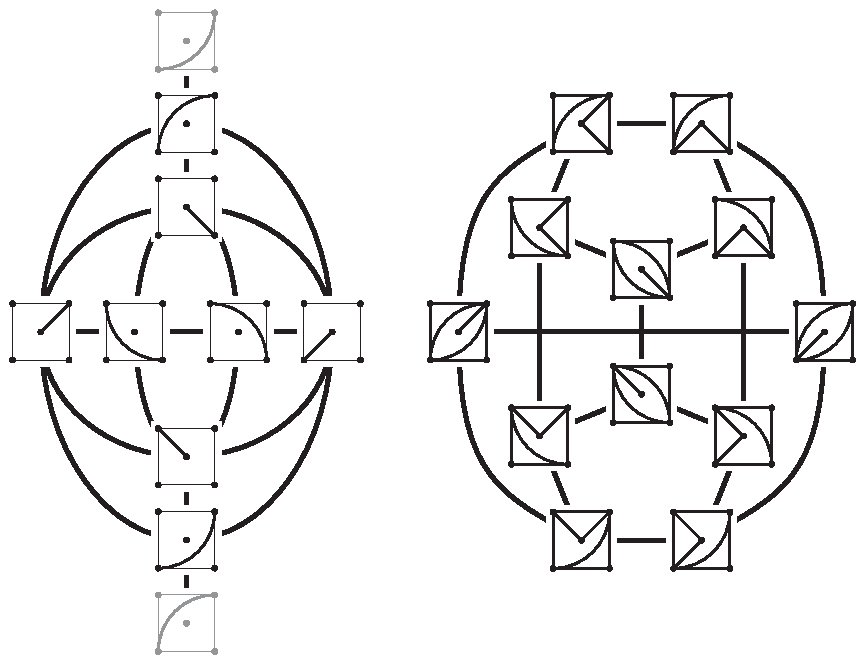
\includegraphics[scale=1]{wigglyComplexSquare}
\caption{The wiggly complex~$\wigglyComplex_P$ (left) and the wiggly flip graph~$\wigglyFlipGraph_P$ (right) of a point set~$P$.}
\label{fig:wigglyComplexSquarre}
\end{figure}
\end{definition}

\begin{conjecture}
\label{conj:polytopality}
For any point set~$P$ in the plane, the wiggly complex~$\wigglyComplex_P$ is the boundary complex of a simplicial polytope.
\end{conjecture}

Note that in \cref{conj:polytopality}, the case of aligned points is given by the wigglyhedron of \cref{thm:wigglyhedron}, while the case of points in general position is given by the pseudotriangulation polytope of~\cite{RoteSantosStreinu-polytope} (see also \cite{RoteSantosStreinu-pseudotriangulations} for a nice survey on pseudotriangulations).

\begin{conjecture}
\label{conj:Hamiltonian2}
For any point set~$P$ in the plane, the wiggly flip graph~$\wigglyFlipGraph_P$ is Hamiltonian.
\end{conjecture}

%%%%%%%%%%%%%%%%%%%%%%%%%%%%%%%%%%%%%%

\section{Further questions}

A few additional questions to arouse your curiosity:
\begin{enumerate}
\item Can the construction of \cref{thm:wigglyhedron} be adapted to provide a more combinatorial construction of the polytope of pseudotriangulations~\cite{RoteSantosStreinu-polytope}, that would only depend on the order type (aka oriented matroid~\cite{BjornerLasVergnasSturmfelsWhiteZiegler}) of the point configuration?
\item What is the dual interpretation of wiggly pseudotriangulations as pseudoline arrangements? (see~\cite{PilaudPocchiola} for context) Can this interpretation be extended to other finite Coxeter groups? (see~\cite{CeballosLabbeStump} for context).
\item What is the multi wiggly complex?
\end{enumerate}


%%%%%%%%%%%%%%%%%%%%%%%%%%%%%%%%%%%%%%

%\clearpage
\addtocontents{toc}{ \vspace{.1cm} }
\bibliographystyle{alpha}
\bibliography{wigglyhedra}
\label{sec:biblio}

\end{document}
